% !TEX root = main.tex
\section{Mathematical proofs}
\label{app:proofs}
The proofs start from \cref{eq:initialization} and use the Euclidean flow in \cref{eq:parameter-flow}.
Throughout, $N\ge4$, $\eta\in[0,\tfrac{1}{2})$, $\gamma=1-2\eta$, $\kappa\in[-1,1]$, and $0<\varepsilon\le1$.
The matrix reduction holds while $|r_1v|<2B$.
The fixed choice in \cref{eq:gate-bound} covers the correlation trajectory through $q=q_1+1$;
trapped trajectories have $r(t)\le \varepsilon$ for all time.
The cross-entropy proof establishes gate validity through complete routing. The causal theorem states its separate gate bound and prefix-size condition.

\subsection{Derivation from the one-block matrices}
\label{app:network-proof}
\label{app:architecture}
\paragraph{Embeddings and attention matrices.}
Let $\bm e_i\in\mathbb R^7$ be standard basis columns and let $\bm0$ denote a zero vector.
The state and query embeddings are
\begin{equation}
 \bm h_j^{(0)}=x_j\bm e_1+\bm e_3+\mathbf1[j=N]\bm e_4+\mathbf1[j<N]\bm e_5,
 \qquad \bm h_q^{(0)}=b\bm e_2+\bm e_3.
 \label{eq:embeddings}
\end{equation}
Here $\mathbf1[\cdot]$ is the indicator of the stated condition.
The one-dimensional query, key and value maps and their output projection are
\begin{equation}
 \begin{gathered}
 \bm w_q=\bm e_3^\top,\qquad
 \bm w_k=q_s\bm e_4^\top+q_d\bm e_5^\top,\qquad
 \bm w_v=\bm e_1^\top,\qquad \bm w_o=\bm e_6,\\
 \bm w_q,\bm w_k,\bm w_v\in\mathbb R^{1\times7},\qquad
 \bm w_o\in\mathbb R^{7\times1}.
 \end{gathered}
 \label{eq:attention-matrices}
\end{equation}
For the $N$ unmasked state positions, define the score vector $\bm q$ and attention vector $\bm\alpha$ by
\begin{equation}
 q_j=(\bm w_q\bm h_q^{(0)})(\bm w_k\bm h_j^{(0)}),\qquad
 \bm\alpha=\softmax(\bm q),\qquad
 \bm h_q=\bm h_q^{(0)}+\bm w_o\sum_{j=1}^N \alpha_j\bm w_v\bm h_j^{(0)}.
 \label{eq:attention-block}
\end{equation}
The query/key dimension is one, so the attention scaling factor is $1$.
The attended value is the scalar $v=\sum_j \alpha_j x_j$; the residual $\bm h_q$ is a vector.

\paragraph{Four-unit MLP matrices.}
Fix $B>0$, let $\bm1_4$ be the four-dimensional all-ones vector, and apply $\relu$ coordinatewise to vector arguments. Set
\begin{equation}
 \begin{gathered}
 \bm w_1=\begin{pmatrix}
 r_1\bm e_6^\top+B\bm e_2^\top\\
 -r_1\bm e_6^\top+B\bm e_2^\top\\
 r_1\bm e_6^\top-B\bm e_2^\top\\
 -r_1\bm e_6^\top-B\bm e_2^\top
 \end{pmatrix},\qquad
 \bm b_1=-B\bm1_4,\\
 \bm w_2=r_2\bm e_7(1,-1,-1,1),\qquad
 \bm w_1\in\mathbb R^{4\times7},\quad
 \bm w_2\in\mathbb R^{7\times4},\quad \bm b_1\in\mathbb R^4,\\
 \bm h'_q=\bm h_q+\bm w_2\relu(\bm w_1\bm h_q+\bm b_1),
 \qquad z=\bm e_7^\top\bm h'_q.
 \end{gathered}
 \label{eq:mlp-matrices}
\end{equation}

\begin{proof}[Proof of \cref{prop:realization}]
\proofstep{(a) Attention.}
For the embeddings and matrices above,
\begin{align*}
 \bm w_q\bm h_q^{(0)}&=1,&
 \bm w_k\bm h_j^{(0)}&=q_s\mathbf1[j=N]+q_d\mathbf1[j<N],&
 \bm w_v\bm h_j^{(0)}&=x_j,\\
 \bm h_q&=\bm h_q^{(0)}+\bm e_6\sum_{j=1}^N \alpha_j x_j,&
 \alpha(q)&=\frac{e^{q_s}}{e^{q_s}+(N-1)e^{q_d}}
 =\frac{e^q}{e^q+N-1}.
\end{align*}
Every decoy has weight $\tfrac{1-\alpha(q)}{N-1}$, so with $\bar w=\tfrac{1}{N-1}\sum_{j<N}x_j$,
\[
 v=\sum_{j=1}^N \alpha_j x_j=\alpha(q)x_N+(1-\alpha(q))\bar w,\qquad |v|\le1.
\]
\proofstep{(b) MLP.}
The preactivation is
\[
 \bm w_1\bm h_q+\bm b_1=
 \begin{pmatrix}
 r_1v+B(b-1)\\-r_1v+B(b-1)\\
 r_1v-B(b+1)\\-r_1v-B(b+1)
 \end{pmatrix}.
\]
Since $\bm e_7^\top\bm h_q=0$ and $|r_1v|<2B$,
\begin{align*}
 b=1:\quad z&=r_2\bigl[\relu(r_1v)-\relu(-r_1v)\bigr]=r_1r_2v,\\
 b=-1:\quad z&=r_2\bigl[-\relu(r_1v)+\relu(-r_1v)\bigr]=-r_1r_2v.
\end{align*}
Thus $z=r_1r_2b v$ on the open gate-valid region.
\proofstep{(c) Parameter gradients.}
For each coordinate $\theta_i$ of $\bm\theta$, differentiation of the identity gives
\begin{align*}
 \pd{}{\theta_i}\E[\ell(y,z)]
 &=\E\left[\pd{\ell}{z}(y,z)\pd{z}{\theta_i}\right]&&\text{(finite support; chain rule)}\\
 &=\E\left[\pd{\ell}{z}(y,r_1r_2b v)\pd{(r_1r_2b v)}{\theta_i}\right]
 =\pd{}{\theta_i}\E[\ell(y,r_1r_2b v)].
\end{align*}
Stacking the four coordinates yields equality of $\nabla_{\bm\theta}$ for the matrix network and its derived logit.
The matrix chain rule, for example, is
\[
 \pd{\mathcal L}{r_1}=\left\langle\nabla_{\bm w_1}\mathcal L,\pd{\bm w_1}{r_1}\right\rangle_{\mathrm F},\qquad
 \pd{\mathcal L}{r_2}=\left\langle\nabla_{\bm w_2}\mathcal L,\pd{\bm w_2}{r_2}\right\rangle_{\mathrm F}.
\]
At $r_1v=0$, the composite $\relu(z)-\relu(-z)=z$ remains differentiable.
Assigning derivative $\tfrac{1}{2}$ to each paired ReLU at zero reproduces its derivative $1$.\qedhere
\end{proof}

\subsection{Cancellation and matched laws}
\label{app:credit-proof}
\begin{proof}[Proof of \cref{lem:credit}]
\proofstep{(a) Factorization.}
Substitute $y=b x_N\xi$:
\begin{align*}
 \E[y b x_j]&=\E[\xi]\E[x_N x_j]=\gamma\E[x_N x_j]
 &&\text{(independence; $b^2=1$)},\\
 \E[y b x_N]&=\gamma
 &&\text{($x_N^2=1$)}.
\end{align*}
\proofstep{(b) Uniform initialization.}
At $\bm q=\bm0$, $\alpha_j=\tfrac{1}{N}$ and
\begin{align*}
 -\pd{\mathcal L}{r_1}
 &=\frac{r_2}{2}\E[y b v]
 =\frac{r_2}{2N}\left(\E[y b x_N]+\sum_{j=1}^{N-1}\E[y b x_j]\right)\\
 &=\frac{r_2\gamma}{2N}\left(1+\sum_{j=1}^{N-1}\E[x_N x_j]\right)
 =\frac{r_2\gamma \kappa}{2N}&&\text{(definition of $\kappa$)}.
\end{align*}
Exchange $r_1,r_2$ for the other rule factor.
Under $\Dlaw{\kappa}$, a decoy is an anti-copy with probability $\tfrac{\E[M]}{N-1}=\rho$ and is otherwise independent of $x_N$, so
$\E[x_N x_j]=-\rho$ and $1+\sum_{j=1}^{N-1}\E[x_N x_j]=1-(N-1)\rho=\kappa$.\qedhere
\end{proof}

\begin{proof}[Proof of \cref{lem:matched}]
\proofstep{(a) Marginals and conditional prediction.}
The law is invariant under the global sign flip $(x_1,\ldots,x_N)\mapsto(-x_1,\ldots,-x_N)$, so every displayed sign is uniform.
Independence of $b,\xi$ from the prefix gives
\begin{align*}
 \Pr(y=b x_N\mid\bm x_{<N+1},b)&=1-\eta,\\
 \Pr(y=-b x_N\mid\bm x_{<N+1},b)&=\eta<\frac{1}{2},\\
 \operatorname*{argmax}_{y\in\{-1,1\}}\Pr(y\mid\bm x_{<N+1},b)&=b x_N.
\end{align*}
\proofstep{(b) One anti-copy.}
The conditional law of $(b,y)$ given the prefix is common to all the laws, so total variation is that of the prefixes;
$x_N$ is uniform under each law, so it is the average over $x_N$ of the total variation of the decoy vectors given $x_N$.
Write $\Dlaw{(m)}$ for the law with exactly $m$ anti-copies and fix $x_N$.
Under $\Dlaw{(0)}=\Dlaw1$ every decoy vector $\bm d\in\{-1,1\}^{N-1}$ has mass $2^{-(N-1)}$.
Under $\Dlaw{(1)}=\Dlaw0$, $\bm d$ arises once for each of its $K(\bm d)$ coordinates equal to $-x_N$, so its mass is
$\tfrac{K(\bm d)}{N-1}2^{-(N-2)}$. With $K$ distributed as under $\Dlaw1$ and $2K-(N-1)=-x_N\sum_{j<N}x_j$,
\[
 d_{\mathrm{TV}}(\Dlaw0,\Dlaw1)=\frac{1}{2}\E_{\Dlaw1}\left|\frac{2K}{N-1}-1\right|
 =\frac{\E|S_{N-1}|}{2(N-1)}=\tau_N\le\frac{\sqrt{N-1}}{2(N-1)},
\]
using $\E|S_{N-1}|\le(\E S_{N-1}^2)^{1/2}$.
The same computation with $N-2$ free decoys compares one further anti-copy with an independent decoy:
$d_{\mathrm{TV}}(\Dlaw{(2)},\Dlaw{(1)})\le\tfrac{1}{2\sqrt{N-2}}$.
\proofstep{(c) Mixtures.}
For $0\le\kappa\le1$, $\Dlaw{\kappa}=\kappa\Dlaw1+(1-\kappa)\Dlaw0$, so
$d_{\mathrm{TV}}(\Dlaw{\kappa},\Dlaw1)=(1-\kappa)\,d_{\mathrm{TV}}(\Dlaw0,\Dlaw1)=(1-\kappa)\tau_N$.
For $-1\le\kappa<0$, $\Dlaw{\kappa}=(1+\kappa)\Dlaw0+(-\kappa)\Dlaw{(2)}$, and the triangle inequality gives
\[
 d_{\mathrm{TV}}(\Dlaw{\kappa},\Dlaw1)\le d_{\mathrm{TV}}(\Dlaw0,\Dlaw1)+(-\kappa)\,d_{\mathrm{TV}}(\Dlaw{(2)},\Dlaw0)
 \le\frac{1-\kappa}{2\sqrt{N-2}}.
\]
\proofstep{(d) Distributional cancellation.}
Under $\Dlaw0$ the multiset of displayed values consists of $x_N$, its anti-copy $-x_N$, and $N-2$ independent uniform signs,
that is, of one $+1$, one $-1$ and $N-2$ independent uniform signs, whatever $x_N$ is.
Hence the multiset is independent of $x_N$; since $b$ and $\xi$ are independent of the prefix, $x_N$ is uniform given $(b,\{x_1,\ldots,x_N\})$,
and so is $y=b x_N\xi$. Under $\Dlaw1$, $\E[y b x_N]=\E[\xi]=\gamma$.\qedhere
\end{proof}

\subsection{From initialization to routing and prediction}
\label{app:flow-proof}
\begin{proof}[Proof of \cref{lem:invariant}]
\proofstep{(a) Balanced trajectory.}
Under $\Dlaw{\kappa}$, $\E[x_N\bar w]=-\rho$ (\cref{lem:credit}), so
$\E[y b v]=\gamma[\alpha(q)-(1-\alpha(q))\rho]=\gamma \phi(q)$. Therefore
\begin{align}
 \mathcal L&=-\frac{\gamma}{2}r_1r_2\phi(q),\notag\\
 \ddt{r_1}&=\frac{\gamma}{2}r_2\phi,&\ddt{r_2}&=\frac{\gamma}{2}r_1\phi,\label{eq:four-scalar-flow}\\
 \ddt{q_s}&=\frac{\gamma}{2}r_1r_2\phi'(q),&
 \ddt{q_d}&=-\frac{\gamma}{2}r_1r_2\phi'(q).\notag
\end{align}
The initialization in \cref{eq:initialization} and uniqueness imply
\begin{align*}
 \frac{d}{dt}(r_1-r_2)&=-\frac{\gamma}{2}\phi(q)(r_1-r_2),&(r_1-r_2)(0)&=0,\\
 \frac{d}{dt}(q_s+q_d)&=0,&(q_s+q_d)(0)&=0.
\end{align*}
Consequently $r_1=r_2=r$, $q_s=-q_d=\tfrac{q}{2}$, and
\begin{equation}
 r(t)=\varepsilon\exp\left(\frac{\gamma}{2}\int_0^t \phi(q(v))\,dv\right)>0,\qquad
 \ddt{q}=\gamma r^2\phi'(q)>0.
 \label{eq:balanced-flow}
\end{equation}
For finite $t$, $|\phi|\le1$, $\phi'(q)\le\tfrac{1+\rho}{4}$ give
\[
 \varepsilon e^{-\frac{\gamma t}{2}}\le r(t)\le \varepsilon e^{\frac{\gamma t}{2}},\qquad
 q(t)\le\frac{\gamma(1+\rho)\varepsilon^2}{4}\int_0^t e^{\gamma v}\,dv<\infty.
\]
These bounds exclude finite-time escape of the derived smooth vector field.
\proofstep{(b) Conserved quantity.}
Set $\alpha_0=\tfrac{\rho}{1+\rho}$ for this calculation only. Then
\begin{align}
 \dv{\alpha(q)}{q}&=\alpha(q)(1-\alpha(q)),&
 \frac{\phi(q)}{\phi'(q)}&=\frac{\alpha(q)-\alpha_0}{\alpha(q)(1-\alpha(q))},\notag\\
 F(q)&=\int_{\tfrac{1}{N}}^{\alpha(q)}\frac{\alpha-\alpha_0}{\alpha^2(1-\alpha)^2}\,d\alpha.\label{eq:primitive}
\end{align}
\begin{align*}
 \frac{d}{dt}(r^2-F(q))
 &=\gamma r^2\phi-\frac{\phi}{\phi'(q)}\gamma r^2\phi'(q)
 &&\text{(chain rule)},\\
 &=0 &&\text{(cancellation)}.
\end{align*}
At initialization $F(0)=0$; hence $r(t)^2=\varepsilon^2+F(q(t))$.
\proofstep{(c) Hitting time.}
If $\varepsilon^2+F>0$ on $[0,b]$, compactness gives
\[
 \min_{0\le q\le b}\gamma(\varepsilon^2+F(q))\phi'(q)>0.
\]
Thus the increasing score gap reaches $b$ in finite time and
\begin{equation}
 T(b)=\int_0^b\frac{dq}{\gamma(\varepsilon^2+F(q))\phi'(q)}.
 \label{eq:hitting-quadrature}
\end{equation}
Taking $b=q_1$ proves \cref{eq:time}.
\proofstep{(d) Gate validity and prediction.}
Since $\alpha_0\ge0$,
\begin{align*}
 \dv{F(q)}{q}&\le\frac{1}{1-\alpha(q)}=1+\frac{e^q}{N-1},\\
 F(q)&\le q+\frac{e^q-1}{N-1}
 <\log(N-1)+1+e\qquad(0\le q\le q_1+1).
\end{align*}
Therefore \cref{eq:gate-bound} gives $|r_1v|\le r<2B$ throughout this interval.
For $\kappa\in\{0,1\}$, $\phi(q)\ge0$ and $F(q)\ge0$ for $q\ge0$; part (c) gives $T(q_1+1)<\infty$.
At $q>q_1$,
\[
 x_N v=\alpha(q)+(1-\alpha(q))x_N\bar w\ge2\alpha(q)-1>0,
 \qquad \operatorname{sign}(z)=b x_N.
\]
Thus the network reaches the Bayes predictor in finite time and retains it through the stopping gap $q_1+1$.\qedhere
\end{proof}

\subsection{Routing-time estimates}
\label{app:routing-proof}
Write $q_1=\log(N-1)$; $N\ge4$ implies $q_1>1$.
The quantitative bounds in parts (i)--(ii) of \cref{thm:separation} are
\begin{align*}
 \frac{N-1}{2e\gamma}\log\!\left(1+\frac{2}{\varepsilon^2}\right)
 &\le\Tr(\Dlaw1)\le\frac{4(N-1)}{\gamma}\left[\log(1+\varepsilon^{-2})+\frac{1}{e}\right],\\
 \frac{N-1}{5\gamma \varepsilon}
 &\le\Tr(\Dlaw0)\le\frac{4(N-1)}{\gamma}\left[\frac{\sqrt2\pi}{\varepsilon}+\frac{8}{e}\right].
\end{align*}

\begin{lemma}[Attention bounds on the routing interval]
\label{lem:attention-bounds}
For $q\in[0,q_1]$,
\begin{equation}
 \frac{e^q}{2(N-1)}\le \alpha(q)\le\frac{e^q}{N},\qquad
 \frac{1}{N}\le \alpha(q)\le\frac{1}{2},\qquad
 \phi'(q)\ge\frac{e^q}{4(N-1)}.
 \label{eq:alpha-bounds}
\end{equation}
For $\kappa\in\{0,1\}$ and $q\in[0,1]$, $\phi'(q)\le \tfrac{e}{N-1}$.
\end{lemma}
\begin{proof}
\begin{align*}
 1\le e^q\le N-1
 &\quad\Longrightarrow\quad
 N\le e^q+N-1\le2(N-1),\\
 \phi'(q)=(1+\rho)\alpha(q)(1-\alpha(q))
 &\ge\frac{\alpha(q)}{2}\ge\frac{e^q}{4(N-1)}&&\text{($\rho\ge0$, $\alpha\le\tfrac12$)},\\
 \kappa\in\{0,1\},\ 0\le q\le1:\quad
 \phi'(q)&\le(1+\rho)\alpha(q)
 \le\frac{N}{N-1}\frac{e^q}{N}\le\frac{e}{N-1}.\qedhere
\end{align*}
\end{proof}

\begin{lemma}[Primitive bounds]
\label{lem:primitive-bounds}
For $0\le q\le q_1$, the two laws satisfy
\begin{align}
 \kappa=1:\quad &q\le F(q)\le2q,\label{eq:ordinary-primitive-bounds}\\
 \kappa=0:\quad &\frac{q^2}{8}\le F(q)\le2q^2\quad(0\le q\le1),\qquad
 F(q)\ge\frac{1}{8}\quad(1\le q\le q_1).
 \label{eq:cancelled-primitive-bounds}
\end{align}
\end{lemma}
\begin{proof}
\proofstep{(a) Ordinary law.}

Here $\rho=0$, $\phi=\alpha$, and $\phi'(q)=\alpha(1-\alpha)$.
\Cref{lem:attention-bounds} gives $1\le \tfrac{\phi}{\phi'(q)}\le2$;
$F(q)=\int_0^q\tfrac{\phi(v)}{\phi'(v)}\,dv\in[q,2q]$.

\proofstep{(b) Cancelled law.}

Here $\rho=\tfrac{1}{N-1}$, and
\[
 \dv{F(q)}{q}=\frac{\alpha(q)-\frac{1}{N}}{\alpha(q)(1-\alpha(q))}\ge0\quad(q\ge0).
\]
For $0\le q\le1$, \cref{lem:attention-bounds} and convexity give
\begin{align*}
 \alpha(q)-\frac{1}{N}
 &=\frac{(e^q-1)(N-1)}{N(e^q+N-1)}\le\frac{e^q-1}{N},\\
 \alpha(q)(1-\alpha(q))&\ge\frac{1}{2N},&
 e^q-1&\le(e-1)q\le2q,\\
 \dv{F(q)}{q}&\le4q,&F(q)&\le2q^2.
\end{align*}
For $0\le q\le q_1$,
\begin{align*}
 \dv{F(q)}{q}&\ge\frac{\alpha(q)-\frac{1}{N}}{\alpha(q)}
 =\frac{N-1}{N}(1-e^{-q})\ge\frac{1}{2}(1-e^{-q}),\\
 0\le q\le1:\quad
 1-e^{-q}&\ge q-\frac{q^2}{2}\ge \frac{q}{2},\\
 F(q)&\ge\int_0^q \frac{v}{4}\,dv=\frac{q^2}{8},\\
 q\ge1:\quad F(q)&\ge F(1)\ge\frac{1}{8}&&\text{($F$ is nondecreasing)}.\qedhere
\end{align*}
\end{proof}

\begin{proof}[Proof of \cref{thm:separation}(i) and \cref{rem:rescaling}]
For a fixed displayed-prefix law and independent error sign, write $\mathcal L_\eta$ for correlation loss. Then
\[
 \mathcal L_\eta(\bm\theta)=(1-2\eta)\mathcal L_0(\bm\theta),\qquad
 \bm\theta_\eta(t)=\bm\theta_0((1-2\eta)t),\qquad
 T(\eta,\kappa)=\frac{T(0,\kappa)}{1-2\eta}.
\]
The trajectory identity follows from the chain rule and uniqueness in the original Euclidean coordinate metric.
It holds on corresponding gate-valid intervals, with infinite routing times interpreted as infinite.
Thus independent corruption at fixed $\kappa=1$ strictly increases finite routing time for $\eta>0$;
the failure threshold at fixed $\kappa<0$ is unchanged.

By \cref{lem:primitive-bounds}, $\varepsilon^2+F(q)>0$ on $[0,q_1]$.
\Cref{lem:invariant,lem:attention-bounds,lem:primitive-bounds} give
\begin{align*}
 \Tr
 &\le\frac{4(N-1)}{\gamma}\int_0^{q_1}\frac{e^{-q}}{\varepsilon^2+q}\,dq\\
 &\le\frac{4(N-1)}{\gamma}
 \left(\int_0^1\frac{dq}{\varepsilon^2+q}+\int_1^\infty e^{-q}\,dq\right)\\
 &=\frac{4(N-1)}{\gamma}\left(\log(1+\varepsilon^{-2})+e^{-1}\right),\\[2pt]
 \Tr
 &\ge\frac{N-1}{e\gamma}\int_0^1\frac{dq}{\varepsilon^2+2q}
 =\frac{N-1}{2e\gamma}\log(1+2\varepsilon^{-2}).\qedhere
\end{align*}
\end{proof}

\begin{proof}[Proof of \cref{thm:separation}(ii)]
By \cref{lem:primitive-bounds}, $\varepsilon^2+F(q)\ge \varepsilon^2>0$.
\Cref{lem:invariant,lem:attention-bounds,lem:primitive-bounds} give
\begin{align*}
 \Tr
 &\ge\frac{N-1}{e\gamma}\int_0^1\frac{dq}{\varepsilon^2+2q^2}
 =\frac{N-1}{e\gamma}\frac{\arctan(\frac{\sqrt2}{\varepsilon})}{\sqrt2\varepsilon}
 \ge\frac{N-1}{\gamma \varepsilon}\frac{\arctan\sqrt2}{\sqrt2e},\\
 \arctan\sqrt2
 &=\int_0^1\frac{dv}{1+v^2}+\int_1^{\sqrt2}\frac{dv}{1+v^2}\\
 &\ge\int_0^1(1-v^2)\,dv+\frac{\sqrt2-1}{3}=\frac{1+\sqrt2}{3},\\
 \sqrt2<\frac{3}{2},\ e<\frac{11}{4}
 &\quad\Longrightarrow\quad
 \frac{\arctan\sqrt2}{\sqrt2e}>\frac{20}{99}>\frac{1}{5},\\[2pt]
 \Tr
 &\le\frac{4(N-1)}{\gamma}
 \left(\int_0^1\frac{dq}{\varepsilon^2+\frac{q^2}{8}}+8\int_1^{q_1}e^{-q}\,dq\right)\\
 &\le\frac{4(N-1)}{\gamma}
 \left(\int_0^\infty\frac{dq}{\varepsilon^2+\frac{q^2}{8}}+8e^{-1}\right)\\
 &=\frac{4(N-1)}{\gamma}
 \left(\frac{\sqrt2\pi}{\varepsilon}+\frac{8}{e}\right).\qedhere
\end{align*}
\end{proof}

\subsection{Diluted cancellation: proof of \texorpdfstring{\cref{cor:dilution}}{the dilution corollary}}
\label{app:dilution}
\begin{proof}[Proof of \cref{cor:dilution}]
For $0\le\lambda\le1$, \cref{def:Dkappa} draws $M\sim\mathrm{Bernoulli}(1-\lambda)$ anti-copies, so $\Dlaw\lambda=\lambda\Dlaw1+(1-\lambda)\Dlaw0$.
Write $\kappa=\lambda$, $\rho=\tfrac{1-\lambda}{N-1}$ and $\alpha_0=\tfrac{\rho}{1+\rho}=\tfrac{1-\lambda}{N-\lambda}$.
\proofstep{(a) The primitive.}
From \cref{eq:primitive}, $F'(q)=\tfrac{\alpha(q)-\alpha_0}{\alpha(q)(1-\alpha(q))}=\tfrac{g(q)}{1-\alpha(q)}$ with
\[
 g(q)=1-\frac{\alpha_0}{\alpha(q)}=\frac{N-1}{N-\lambda}\Bigl[\lambda+(1-\lambda)(1-e^{-q})\Bigr]\ge0 .
\]
On $[0,q_1]$, $1\le\tfrac{1}{1-\alpha(q)}\le2$, and $\tfrac{N-1}{N-\lambda}\in[\tfrac{3}{4},1]$. For $0\le q\le1$, $\tfrac{q}{2}\le1-e^{-q}\le q$, and
$\lambda+(1-\lambda)q\ge\tfrac{\lambda+q}{4}$ (if $\lambda\le\tfrac12$ the left side is at least $\lambda+\tfrac{q}{2}$; otherwise it is at least $\lambda>\tfrac12\ge\tfrac{\lambda+q}{4}$). Hence
\[
 \frac{3}{32}(\lambda+q)\le F'(q)\le2(\lambda+q),\qquad
 \frac{3}{32}\Bigl(\lambda q+\frac{q^2}{2}\Bigr)\le F(q)\le2\Bigl(\lambda q+\frac{q^2}{2}\Bigr)\qquad(0\le q\le1),
\]
and, since $F$ is nondecreasing, $F(q)\ge F(1)\ge\tfrac{3}{64}$ on $[1,q_1]$.
\proofstep{(b) Time bounds.}
\Cref{lem:attention-bounds} gives $\phi'(q)\ge\tfrac{e^q}{4(N-1)}$ on $[0,q_1]$, and its upper bound $\phi'(q)\le(1+\rho)\alpha(q)\le\tfrac{e}{N-1}$ on $[0,1]$ holds for every $\lambda\in[0,1]$ because $1+\rho\le\tfrac{N}{N-1}$.
Write $I=\int_0^1\tfrac{dq}{\varepsilon^2+\lambda q+q^2}$; note $I\ge\tfrac{1}{3}$. Using $\varepsilon^2+F\le2(\varepsilon^2+\lambda q+q^2)$ and $\varepsilon^2+F\ge\tfrac{3}{64}(\varepsilon^2+\lambda q+q^2)$ on $[0,1]$, \cref{eq:time} gives
\begin{align*}
 \Tr&\ge\frac{N-1}{e\gamma}\int_0^1\frac{dq}{\varepsilon^2+F(q)}\ge\frac{N-1}{2e\gamma}\,I,\\
 \Tr&\le\frac{4(N-1)}{\gamma}\left(\int_0^1\frac{e^{-q}\,dq}{\varepsilon^2+F(q)}+\int_1^{q_1}\frac{e^{-q}\,dq}{F(1)}\right)\\
 &\le\frac{256(N-1)}{3\gamma}\bigl(I+e^{-1}\bigr)\le\frac{256(1+3e^{-1})(N-1)}{3\gamma}\,I .
\end{align*}
\proofstep{(c) The integral.}
Since $\max\{a,b,c\}\le a+b+c\le3\max\{a,b,c\}$, $I$ is within a factor $3$ of $J=\int_0^1\tfrac{dq}{\max\{\varepsilon^2,\lambda q,q^2\}}$.
If $\lambda\le\varepsilon$, then $\lambda q\le\max\{\varepsilon^2,q^2\}$ and $J=\tfrac{2}{\varepsilon}-1\in[\tfrac{1}{\varepsilon},\tfrac{2}{\varepsilon}]$.
If $\lambda>\varepsilon$, the three regimes meet at $q=\tfrac{\varepsilon^2}{\lambda}<\lambda\le1$, and
\[
 J=\frac{1}{\lambda}+\frac{2}{\lambda}\log\frac{\lambda}{\varepsilon}+\frac{1}{\lambda}-1
 \in\left[\frac{1+2\log(\lambda/\varepsilon)}{\lambda},\ \frac{2+2\log(\lambda/\varepsilon)}{\lambda}\right].
\]
With $C=\tfrac{1+\log(1+\lambda/\varepsilon)}{\lambda}$: for $\lambda\le\varepsilon$, $C\ge\tfrac{1}{\lambda}\ge\tfrac{1}{\varepsilon}$, so $\min\{\tfrac{1}{\varepsilon},C\}=\tfrac{1}{\varepsilon}$;
for $\lambda>\varepsilon$, $\log\tfrac{\lambda}{\varepsilon}\le\log(1+\tfrac{\lambda}{\varepsilon})\le\log\tfrac{\lambda}{\varepsilon}+\log2$ and $C\le\tfrac{1+\log2}{\varepsilon}$.
In both cases $J$, and hence $I$, is within absolute constants of $\min\{\tfrac{1}{\varepsilon},C\}$; with part (b) this proves the corollary.
\end{proof}
Numerically, $F(q)/(\lambda q+\tfrac{q^2}{2})\in[0.67,1.14]$ on $[0,1]$ for $N\in\{8,16,64,256\}$, and
$\tfrac{\gamma\Tr}{(N-1)I}\in[1.03,1.51]$ over $N\in\{16,64\}$, $\varepsilon\in\{10^{-2},10^{-3},10^{-4}\}$ and eleven values of $\lambda\in[0,1]$, well inside the proved constants.

\subsection{Over-cancellation: exact barrier and critical equality}
\label{app:critical}

\begin{lemma}[Barrier location and size]
\label{lem:barrier}
For $-1\le \kappa<0$, let $\alpha_0=\tfrac{1+|\kappa|}{N+|\kappa|}$ and $q_0=\log(1-\kappa)$.
Then $\phi(q_0)=0$, $\alpha(q_0)=\alpha_0$, and
\begin{equation}
 \min_{q\ge0}F(q)=F(q_0)<0,\qquad
 \frac{9\kappa^2}{200}\le -F(q_0)\le2\kappa^2,\qquad
 \frac{1}{N}<\alpha_0\le\frac{2}{N}.
 \label{eq:barrier-bounds}
\end{equation}
\end{lemma}
\begin{proof}
\proofstep{(a) Location and sign.}
\begin{align*}
 \frac{(N-1)\alpha_0}{1-\alpha_0}&=(N-1)\rho=1-\kappa,\\
 \dv{F(q)}{q}&=\frac{\alpha(q)-\alpha_0}{\alpha(q)(1-\alpha(q))},\\
 q<q_0&\Rightarrow \dv{F(q)}{q}<0,&q>q_0&\Rightarrow \dv{F(q)}{q}>0,\\
 |\kappa|(N-2)\le N&\Rightarrow \alpha_0\le\frac{2}{N}.
\end{align*}
\proofstep{(b) Lower bound.}
\begin{align*}
 -F(q_0)
 &=\int_{\frac{1}{N}}^{\alpha_0}\frac{\alpha_0-\alpha}{\alpha^2(1-\alpha)^2}\,d\alpha
 \ge\frac{(\alpha_0-\frac{1}{N})^2}{2\alpha_0^2}
 =\frac{(N \alpha_0-1)^2}{2(N \alpha_0)^2},\\
 N \alpha_0-1&=\frac{|\kappa|(N-1)}{N+|\kappa|}\ge\frac{3}{5}|\kappa|,&N \alpha_0&\le2,\\
 -F(q_0)&\ge\frac{9\kappa^2}{200}.
\end{align*}
\proofstep{(c) Upper bound.}
For $\alpha\in[\tfrac{1}{N},\alpha_0]$,
\begin{align*}
 \alpha^2(1-\alpha)^2&\ge\frac{(1-\alpha_0)^2}{N^2}\ge\frac{1}{4N^2},\\
 -F(q_0)&\le4N^2\int_{\frac{1}{N}}^{\alpha_0}(\alpha_0-\alpha)\,d\alpha
 =2(N \alpha_0-1)^2\le2\kappa^2.\qedhere
\end{align*}
\end{proof}

The failure part also yields the following quantitative conclusions.
Below this barrier, $q(t)\uparrow q_z<q_0$ and $r(t)\to0$, where $q_z$ is the unique root of $\varepsilon^2+F(q_z)=0$.
At equality, $q(t)\uparrow q_0$ and $r(t)\downarrow0$.
Both failure cases have $\alpha(q(t))<\tfrac{2}{N}$ for every finite $t$.
Moreover $\tfrac{9\kappa^2}{200}\le-F(q_0)\le2\kappa^2$;
$\varepsilon\le\tfrac{|\kappa|}{9}$ suffices for failure, and $\varepsilon>\sqrt2|\kappa|$ suffices for routing.
\begin{proof}[Proof of \cref{thm:separation}(iii)]
\proofstep{(a) Above the barrier.}
If $\varepsilon^2>-F(q_0)$, then $\min_{[0,q_1]}(\varepsilon^2+F)>0$ by \cref{lem:barrier}; \cref{lem:invariant} gives $\Tr<\infty$.
\proofstep{(b) Below the barrier.}

\Cref{lem:barrier} gives strict decrease of $F$ on $[0,q_0]$, with
$\varepsilon^2+F(0)>0>\varepsilon^2+F(q_0)$; hence $q_z$ exists uniquely.
By \cref{lem:invariant},
\[
 r(t)>0,\qquad r(t)^2=\varepsilon^2+F(q(t)),\qquad\ddt{q}>0
 \quad\Longrightarrow\quad 0\le q(t)<q_z.
\]
Let $q_\infty=\lim_{t\to\infty}q(t)\le q_z$.
If $q_\infty<q_z$, then
\[
 \ddt{q}(t)\ge\min_{0\le q\le q_\infty}
 \gamma(\varepsilon^2+F(q))\phi'(q)>0,
\]
so $q(t)\to\infty$, a contradiction. Therefore $q_\infty=q_z$ and
$r(t)^2\to \varepsilon^2+F(q_z)=0$.

\proofstep{(c) Equality.}

At $q=q_0$, $\phi=0$ and
\begin{align*}
 \left.\dv{F(q)}{q}\right|_{q=q_0}&=0,\\
 \left.\frac{d^2F(q)}{dq^2}\right|_{q=q_0}
 &=\left.\dv{}{q}\left(\frac{\phi(q)}{\phi'(q)}\right)\right|_{q=q_0}\\
 &=\left.\left[1-\frac{\phi(q)\phi''(q)}{\bigl(\phi'(q)\bigr)^2}\right]\right|_{q=q_0}=1.
\end{align*}
Taylor's theorem gives $b>0$ such that, for $q_0-b\le q\le q_0$,
\[
 \frac{1}{4}(q-q_0)^2\le F(q)-F(q_0)\le\frac{3}{4}(q-q_0)^2.
\]
On $[0,q_0]$, $\phi'(q)\le\tfrac{1+\rho}{4}$, so
\[
 \int_{q_0-b}^{q_0}\frac{dq}{\gamma[\varepsilon^2+F(q)]\phi'(q)}
 \ge\frac{16}{3\gamma(1+\rho)}\int_{q_0-b}^{q_0}\frac{dq}{(q-q_0)^2}=\infty.
\]
Thus $q(t)<q_0$ at every finite time.
The same bounded-monotone limit argument as in part (b) yields
$q(t)\uparrow q_0$ and $r(t)^2\to \varepsilon^2+F(q_0)=0$.
Since $\phi(q)<0$ for $q<q_0$, $\ddt{r}<0$.
\proofstep{(d) Attention and sufficient conditions.}
Finally $q_0=\log(1-\kappa)\le\log2<\log(N-1)=q_1$, so routing fails. In both failure cases $\alpha(q(t))<\alpha(q_0)=\alpha_0\le\tfrac{2}{N}$.
The bounds in \cref{lem:barrier} give
\[
 \varepsilon\le\frac{|\kappa|}{9}\ \Longrightarrow\ \varepsilon^2<\frac{9\kappa^2}{200}\le-F(q_0),\qquad
 \varepsilon>\sqrt2|\kappa|\ \Longrightarrow\ \varepsilon^2>2\kappa^2\ge-F(q_0).\qedhere
\]
\end{proof}

\subsection{Cross-entropy: escape from uniform attention}
\label{app:ce-proof}
Write $u=x_N\bar w\in[-1,1]$, so that $x_N v=s(q,u):=\alpha(q)+(1-\alpha(q))u$ and $\E[u]=-\rho$.
For the original coordinate metric, the exact balanced cross-entropy flow is
\begin{align}
 \ddt{r}&=\frac{r}{2} f(q,r^2),\qquad \ddt{q}=r^2j(q,r^2),\label{eq:ce-flow}\\
 f(q,m)&=\gamma \phi(q)-\E\left[s\tanh\!\left(\frac{m s}{2}\right)\right],\notag\\
 j(q,m)&=\alpha(q)(1-\alpha(q))\,\E\left[(1-u)\left(\gamma-\tanh\!\left(\frac{m s}{2}\right)\right)\right],\notag
\end{align}
with $s=s(q,u)$ inside the expectations.
Here $m$ is a scalar argument; the trained parameters remain $\bm\theta$.
The factor two in the score-gap velocity comes from training both the source score and the shared decoy score.
It is absent if only one gap parameter is trained.
For a two-valued read, $u\in\{-1,1\}$, the factor $1-u$ removes the state $s=1$ and the remaining state has $s=2\alpha-1\le0$ before routing,
so then $j\ge\gamma\phi'(q)$. The anti-copy read takes many values in $[-1,1]$; we only use $|j-\gamma\phi'(q)|\le\tfrac{m}{2}\phi'(q)$,
which keeps $j$ positive while $m<2\gamma$.

\begin{proof}[Proof of \cref{thm:separation}(iv)]
Fix $N,\gamma$ and $\kappa\in\{0,1\}$. Constants below depend on $N,\gamma$, but not on $\varepsilon$.
\proofstep{(a) Exact loss derivatives.}
Write $m=r_1r_2$ inside this proof; then $y z=\xi m s$.
Averaging over the independent error sign, $\E_\xi[\xi\sigma(-\xi a)]=\tfrac{1}{2}(\gamma-\tanh\tfrac{a}{2})$ for the logistic function $\sigma$, so
\begin{align*}
 \pd{\mathcal L_{\mathrm{ce}}}{m}
 &=-\frac{1}{2}\E\left[s\left(\gamma-\tanh\!\left(\frac{m s}{2}\right)\right)\right]
 =-\frac{f(q,m)}{2},\\
 \pd{\mathcal L_{\mathrm{ce}}}{q}
 &=-\frac{m}{2}\E\left[\pd{s}{q}\left(\gamma-\tanh\!\left(\frac{m s}{2}\right)\right)\right]
 =-\frac{m j(q,m)}{2},
\end{align*}
since $\E[s]=\phi(q)$ and $\pd{s}{q}=\alpha(q)(1-\alpha(q))(1-u)$.
The coordinate flow therefore satisfies
\begin{align*}
 \ddt{r_1}&=\frac{r_2f}{2},&\ddt{r_2}&=\frac{r_1f}{2},\\
 \frac{d}{dt}(r_1-r_2)&=-\frac{f}{2}(r_1-r_2),&(r_1-r_2)(0)&=0,\\
 \ddt{q_s}&=\frac{m j}{2},&\ddt{q_d}&=-\frac{m j}{2}.
\end{align*}
Hence $r_1=r_2=r$, $m=r^2$, $q_s=-q_d=\tfrac{q}{2}$, and
\[
 \ddt{r}=\frac{r f}{2},\qquad \ddt{q}=m j,\qquad
 \ddt{m}=m f,\qquad (m(0),q(0))=(\varepsilon^2,0).
\]
\proofstep{(b) Uniform nonlinear bound.}
Using $|\tanh z|\le|z|$, $|s|\le1$, $1-u\ge0$ and $\E[1-u]=1+\rho$,
\begin{align*}
 |f-\gamma \phi|&\le\frac{m}{2}\E[s^2]\le\frac{m}{2},\\
 \left|j-\gamma\phi'(q)\right|&\le\frac{m}{2}\alpha(q)(1-\alpha(q))\E[1-u]=\frac{m}{2}\phi'(q).
\end{align*}
Choose a small fixed $b_0\in(0,\min(1,q_1))$.
Since $\phi'(q)>0$ on its compact closure, there is one constant $C\ge1$ such that
\begin{equation}
 \frac{1}{C}\le j(q,m)\le C,\qquad
 \left|\frac{f(q,m)}{j(q,m)}-\frac{\phi(q)}{\phi'(q)}\right|\le Cm
 \quad(0\le q\le b_0,\ 0\le m\le\gamma).
 \label{eq:ce-ratio-bound}
\end{equation}
Indeed $\tfrac{\gamma}{2}\phi'(q)\le j\le(\gamma+\tfrac{1}{2})\phi'(q)$ for $m\le\gamma$, and the second bound follows from
\[
 \left|\frac{f}{j}-\frac{\phi}{\phi'(q)}\right|
 \le\frac{|f-\gamma \phi|}{j}
 +\left|\frac{\phi}{\phi'(q)}\right|\frac{|\gamma\phi'(q)-j|}{j}.
\]
\proofstep{(c) Score-parametrized comparison.}
For $\kappa=1$, $\tfrac{\phi}{\phi'(q)}=\tfrac{1}{1-\alpha}\in[1,2]$.
For $\kappa=0$, $\phi(0)=0$ and
\[
 \left.\dv{}{q}\left(\frac{\phi(q)}{\phi'(q)}\right)\right|_{q=0}=1.
\]
After decreasing $b_0$, both laws satisfy
\[
 \frac{1}{2}q^{1-\kappa}\le\frac{\phi(q)}{\phi'(q)}\le2q^{1-\kappa}.
\]
For $\kappa=1$, $q^{1-\kappa}$ here means the constant function $1$, including at $q=0$.
While $m\le\gamma$, $j>0$ and \cref{eq:ce-ratio-bound} gives
\[
 \frac{1}{2}q^{1-\kappa}-Cm\le\dv{m}{q}=\frac{f}{j}\le2q^{1-\kappa}+Cm.
\]
Multiplying by the integrating factors $e^{Cq}$ and $e^{-Cq}$ and integrating from zero yields
\begin{align*}
 m(q)&\ge e^{-Cq}\left(\varepsilon^2+\frac{1}{2}\int_0^q e^{Cv}v^{1-\kappa}\,dv\right),\\
 m(q)&\le e^{Cq}\left(\varepsilon^2+2\int_0^q e^{-Cv}v^{1-\kappa}\,dv\right).
\end{align*}
Thus for $0\le q\le b\le b_0$, as long as $m\le\gamma$ on $[0,q]$,
\begin{equation}
 \frac{e^{-Cb}}{4}(\varepsilon^2+q^{2-\kappa})\le m(q)
 \le2e^{Cb}(\varepsilon^2+q^{2-\kappa}).
 \label{eq:ce-polynomial-comparison}
\end{equation}
\proofstep{(d) Existence, gate validity, and time.}
Choose $b\in(0,b_0)$ and $\varepsilon_0\le1$ sufficiently small that
$2e^{Cb}(\varepsilon_0^2+b^{2-\kappa})<\min\{\gamma,4B^2\}$.
By the upper bound in part (c), the first time $m$ could reach $\gamma$ or the gate value $4B^2$ would already have $m<\min\{\gamma,4B^2\}$,
a contradiction, so neither happens before $q=b$; the lower bound prevents exit through $m=0$.
The smooth equation $\dv{m}{q}=\tfrac{f}{j}$ therefore extends to $q=b$.
Define
\[
 T(q)=\int_0^q\frac{dv}{m(v)j(v,m(v))}.
\]
This finite, strictly increasing map reconstructs the initialized network flow:
$\ddt{q}=m j$, $\ddt{m}=m f$, $r=\sqrt m$, $q_s=-q_d=\tfrac{q}{2}$.
Uniqueness and the gate bound identify it with \cref{eq:parameter-flow}.
Combining \cref{eq:ce-ratio-bound,eq:ce-polynomial-comparison} gives
\begin{equation}
 \frac{e^{-Cb}}{2C}\int_0^b\frac{dq}{\varepsilon^2+q^{2-\kappa}}
 \le T(b)\le4Ce^{Cb}\int_0^b\frac{dq}{\varepsilon^2+q^{2-\kappa}}.
 \label{eq:ce-hitting-bounds}
\end{equation}
Finally,
\begin{align*}
 \kappa=1:\quad\int_0^b\frac{dq}{\varepsilon^2+q}
 &=\log\!\left(1+\frac{b}{\varepsilon^2}\right)=\Theta\!\left(\log\!\frac{1}{\varepsilon}\right),\\
 \kappa=0:\quad\int_0^b\frac{dq}{\varepsilon^2+q^2}
 &=\frac{1}{\varepsilon}\arctan\!\left(\frac{b}{\varepsilon}\right)=\Theta\!\left(\frac{1}{\varepsilon}\right).
\end{align*}
Set $q_{\mathrm{esc}}=b$; these are the escape-time orders.\qedhere
\end{proof}

\paragraph{Beyond the escape gap.}
The two-valued argument continued to routing using $j\ge\gamma\phi'(q)$ on all of $[0,q_1]$.
For the anti-copy read this lower bound is only available while $m<2\gamma$, and along the numerical trajectories $m$ exceeds $2\gamma$ before routing.
Numerical integration of \cref{eq:ce-flow} for $N\in\{16,64\}$, $\eta=0.1$, $\kappa\in\{1,0\}$ and $\varepsilon\in[10^{-4},0.03]$ shows that
routing completes in every case, and $j$ stays above $0.04$ ($N=16$) and $0.005$ ($N=64$) along every trajectory.
At $q>q_1$ any positive rule product gives $\operatorname{sign}(z)=b x_N$, as in \cref{app:flow-proof}.

\paragraph{A finite-initialization correction.}
Under $\Dlaw0$, the correlation contribution to the rule gradient is zero at $q=0$.
For $r>0$, cross-entropy instead gives $f(0,r^2)<0$, with expansion
\[
 f(0,r^2)=-\frac{r^2}{2}\E[v(0)^2]+O(r^6).
\]
Thus $\ddt{r}$ initially shrinks at order $r^3$, even though the leading credit cancels.
This correction is compatible with the routing theorem's local comparison: it changes the comparison by $O(r^2)$ without removing the quadratic growth in the score gap.

\subsection{Full-matrix plateau: proof of \texorpdfstring{\cref{thm:fullmatrix}}{the full-matrix theorem}}
\label{app:fullmatrix}
Throughout, $\|\cdot\|$ is the Euclidean norm for vectors and the operator norm for matrices, bounded by the Frobenius norm;
$\|W-W_0\|_F\le\varepsilon$ bounds the deviation of every block, $\delta Q=Q-Q_0$ and so on. The state embeddings satisfy $\|s_j\|=\sqrt3$,
the query embedding $h_b=b\bm e_2+\bm e_3$ satisfies $\|h_b\|=\sqrt2$, and $0<\varepsilon\le\tfrac{1}{10}$, $B\ge1$.
Write $u=\tfrac{1}{N}\bm1$, $\bar s=\sum_j u_js_j$, $H_b=\sum_j\alpha_j(b)s_j$ and $M=OV$.
The embeddings and $W_0$ are padded with zeros from $\mathbb R^7$ to $\mathbb R^{d_{\mathrm{res}}}$; padding changes none of the norms and products used below,
and every perturbation bound uses operator norms dominated by $\|W-W_0\|_F$, so no bound depends on $d_{\mathrm{res}}$, $d$, $d_v$ or $m$.

\begin{proof}[Proof of \cref{thm:fullmatrix}]
\proofstep{(a) Uniform attention carries no rule credit.}
Let $z^{\mathrm{u}}_W$ be the logit with every attention weight replaced by $\tfrac1N$ and all matrices kept.
It is a function of $b$ and of $\bar s=\tfrac{S}{N}\bm e_1+\bm e_3+\tfrac1N\bm e_4+\tfrac{N-1}{N}\bm e_5$, where $S$ is the sum of the displayed values,
which is a function of their multiset. By \cref{lem:matched}, $x_N$ is uniform given $(b,\bar s)$ under $\Dlaw0$; since $\xi$ is independent of everything else,
$\E[yz^{\mathrm u}_W]=\gamma\,\E\bigl[b\,z^{\mathrm u}_W\,\E[x_N\mid b,\bar s]\bigr]=0$, and $\E[yz_W]=\gamma\,\E[b\,x_N(z_W-z^{\mathrm u}_W)]$.
\proofstep{(b) Attention stays almost uniform and almost instruction-blind.}
The score of position $j$ is $\sigma_j(b)=(Qh_b)^\top Ks_j$. Since $K_0=0$, $Q_0h_b=\bm e_1$ and $Q_0\bm e_2=0$,
\[
 |\sigma_j(b)|\le(1+\sqrt2\varepsilon)\,\varepsilon\sqrt3\le2.1\varepsilon,\qquad
 |\sigma_j(1)-\sigma_j(-1)|=2|(\delta Q\,\bm e_2)^\top Ks_j|\le2\sqrt3\varepsilon^2\le3.5\varepsilon^2 .
\]
If all scores lie in $[-m,m]$ with $m\le0.34$, every weight lies in $[\tfrac{e^{-2m}}{N},\tfrac{e^{2m}}{N}]$, so $\|\bm\alpha-u\|_1\le e^{2m}-1\le4m$;
the softmax Jacobian $\operatorname{diag}(\bm\alpha)-\bm\alpha\bm\alpha^\top$ maps $\ell_\infty$ into $\ell_1$ with norm at most $2$. Hence
\[
 \|H_b-\bar s\|\le\sqrt3\cdot8.4\varepsilon\le15\varepsilon,\qquad
 \|H_1-H_{-1}\|\le\sqrt3\cdot7\varepsilon^2\le12.2\varepsilon^2 .
\]
\proofstep{(c) Three small products.}
At initialization $c_0^\top O_0=\bm e_7^\top\bm e_6=0$, $\|U_0O_0\|=\|U_0\bm e_6\|=2\varepsilon$, $\|c_0^\top D_0\|=2\varepsilon$, $\|U_0\|\le2B+0.2$ and $\|V\|\le1.1$.
Expanding each product to first order in the deviations,
\begin{align*}
 \|c^\top M\|&\le1.1\bigl(\|c_0^\top\delta O\|+\|\delta c^\top O_0\|+\|\delta c^\top\delta O\|\bigr)\le2.4\varepsilon,\\
 \|UM\|&\le1.1\bigl(\|U_0O_0\|+\|U_0\|\|\delta O\|+\|\delta U\|+\|\delta U\|\|\delta O\|\bigr)\le(2.2B+3.7)\varepsilon,\\
 \|c^\top D\|&\le\|c_0^\top D_0\|+\|\delta D\|+\|\delta c\|\|D_0\|+\|\delta c\|\|\delta D\|\le3.3\varepsilon .
\end{align*}
\proofstep{(d) The credit bound.}
With $g_b=h_b+MH_b$ and $\bar g_b=h_b+M\bar s$,
\[
 z_W-z^{\mathrm u}_W=c^\top M(H_b-\bar s)+c^\top D\bigl[\relu(Ug_b+a)-\relu(U\bar g_b+a)\bigr].
\]
The instruction $b$ is uniform and independent of the prefix, and $\bar s$ does not depend on $b$, so the first term contributes
$\tfrac12\E[x_N\,c^\top M(H_1-H_{-1})]$, at most $\tfrac12\cdot2.4\varepsilon\cdot12.2\varepsilon^2\le14.7\varepsilon^3$ in absolute value.
Since $\relu$ is $1$-Lipschitz coordinatewise, the second term is at most $\|c^\top D\|\,\|UM\|\,\|H_b-\bar s\|\le3.3\cdot15\,(2.2B+3.7)\,\varepsilon^3$.
Together, $|\E[yz_W]|\le\gamma(109B+198)\varepsilon^3\le\gamma C_B\varepsilon^3$, which is (i).
For the loss, $\log(1+e^{-yz})=\log2-\tfrac{yz}{2}+\log\cosh\tfrac{z}{2}$ and $\log\cosh\ge0$ give $\mathcal L(W)\ge\log2-\tfrac12\E[yz_W]$.
\proofstep{(e) Initial loss.}
At $W_0$ the network is the four-scalar network at $\bm\theta(0)$, so $z_{W_0}=\varepsilon^2bv$ with uniform attention and $|z_{W_0}|\le\varepsilon^2$.
By part (a), $\E[yz_{W_0}]=0$, and $\log\cosh x\le\tfrac{x^2}{2}$ gives $\mathcal L(W_0)\le\log2+\tfrac{\varepsilon^4}{8}$.
\proofstep{(f) Energy and first exit.}
The population loss is a finite sum of compositions of affine maps, $\exp$, $\log$ and $\relu$, so it is locally Lipschitz and definable in the o-minimal structure $\mathbb R_{\exp}$.
Along any absolutely continuous solution of $\dot W\in-\partial\mathcal L(W)$ the chain rule for definable locally Lipschitz functions \citep{davis2020stochastic} gives
$\tfrac{d}{dt}\mathcal L(W(t))=-\|\dot W(t)\|_F^2$ for almost every $t$, hence, by Cauchy--Schwarz,
\[
 \|W(t)-W(0)\|_F^2\le t\int_0^t\|\dot W\|_F^2=t\,\bigl[\mathcal L(W(0))-\mathcal L(W(t))\bigr].
\]
Let $\tau$ be the first time $\|W(t)-W_0\|_F=\varepsilon$. On $[0,\tau]$ part (d) applies, so $\mathcal L(W_0)-\mathcal L(W(t))\le\tfrac{\varepsilon^4}{8}+\tfrac{\gamma C_B\varepsilon^3}{2}\le C_B\varepsilon^3$.
At $t=\tau$ this gives $\varepsilon^2\le\tau C_B\varepsilon^3$, that is $\tau\ge\tfrac{1}{C_B\varepsilon}$, which is (ii).
\proofstep{(g) Small perturbations.}
On the ball $\|W-W_0\|_F\le\varepsilon$ every factor in the network is bounded by a constant depending only on $B$, so $z_W$ is Lipschitz in $W$ there with a constant $L_B$.
If $\|W(0)-W_0\|_F\le\varepsilon^{3/2}$, then $|z_{W(0)}|\le\varepsilon^2+L_B\varepsilon^{3/2}$ and, by part (d),
$\mathcal L(W(0))\le\log2+\tfrac{\gamma C_B\varepsilon^3}{2}+\tfrac{(1+L_B)^2\varepsilon^3}{8}$.
Since $\varepsilon^{3/2}\le\tfrac{\varepsilon}{2}$, the ball of radius $\tfrac{\varepsilon}{2}$ around $W(0)$ lies inside the ball of part (d), and the argument of part (f) gives exit time at least
$\tfrac{(\varepsilon/2)^2}{C'_B\varepsilon^3}$ with $C'_B=C_B+(1+L_B)^2$, which is (iii).\qedhere
\end{proof}

\subsection{Causal, constant-rate error cancellation}
\label{app:trace-proof}
\begin{proof}[Proof of \cref{thm:causal}]
\proofstep{(a) A valid error process.}
Write $S_i=\sum_{j=1}^i x_j$ and $V_i=N^2+N-i$ inside this proof.
For $N\le i\le2N$,
\[
 \frac{|x_i S_i|}{V_i}\le\frac{2N}{N^2-N}=\frac{2}{N-1}<\min\{2\eta,\gamma\}.
\]
Thus every conditional error probability in \cref{eq:causal-kernel} lies strictly between $0$ and $\tfrac{1}{2}$.
The Bayes predictor given the entire prefix and instruction is therefore $b_{i+1}x_i$ in both regimes.
The prescribed kernel depends only on the displayed past and current instruction, so the process is causal.
\proofstep{(b) Moments created by the error kernel.}
In the cancelling regime,
\begin{align*}
 \E[\xi_{i+1}\mid\bm x_{<i+1},b_{i+1}]&=\gamma-\frac{b_{i+1}x_i S_i}{V_i},\\
 \E[x_{i+1}\mid\bm x_{<i+1}]
 &=\frac{1}{2}\sum_{b=\pm1}b x_i\left(\gamma-\frac{b x_i S_i}{V_i}\right)
 =-\frac{S_i}{V_i}.
\end{align*}
At the seed, $\E[S_N^2]=N^2=V_N$. Inductively,
\begin{align*}
 \E[x_{i+1}S_i]&=-\frac{\E[S_i^2]}{V_i}=-1&&\text{(conditioning; induction)},\\
 \E[S_{i+1}^2]&=\E[S_i^2]+2\E[x_{i+1}S_i]+1
 =V_i-1=V_{i+1} &&\text{(definition of $V_i$)},\\
 \E[x_{i+1}S_{i+1}]&=\E[x_{i+1}S_i]+1=0&&\text{($x_{i+1}^2=1$)}.
\end{align*}
Global sign reversal preserves the kernel and reverses the displayed states.
Hence $\E[x_i]=\E[S_i]=0$ and each $x_i$ is uniform.
For $i\ge N+1$, the last identity gives
\[
 \E[S_i\mid x_i=1]=\E[S_i\mid x_i=-1]=0.
\]
Since the next instruction is independent of the prefix, averaging the error kernel conditional on $(x_i,b_{i+1})$ gives exactly $\eta$.
Also $\E[x_i(S_i-x_i)]=-1$, proving cancellation at every supervised position.
In the independent-error regime, a fresh uniform instruction makes $x_{i+1}$ uniform independently of its entire displayed past;
therefore $\E[x_i(S_i-x_i)]=0$ at the supervised positions.
Averaging either error kernel over its fresh instruction gives error probability $\eta$ at each of the $N+1$ noisy transitions.
The other $N-1$ transitions are correct; the expected incorrect fraction is $\tfrac{\eta(N+1)}{2N}$.
\proofstep{(c) High-probability corruption.}
Let $\mathcal F_i$ be the history generated by $(w,b_2,\xi_2,\ldots,b_i,\xi_i)$ immediately before drawing $b_{i+1}$,
with $\xi_2=\cdots=\xi_N=1$, and put $I_{i+1}=\mathbf 1\{\xi_{i+1}=-1\}$.
In either regime, averaging the fresh uniform instruction gives
\[
 \Pr(I_{i+1}=1\mid\mathcal F_i)
 =\frac{1}{2}\sum_{b=\pm1}\Pr(\xi_{i+1}=-1\mid\mathcal F_i,b_{i+1}=b)=\eta.
\]
For any $a_{N+1},\ldots,a_{2N+1}\in\{0,1\}$, repeated conditioning therefore yields
\[
 \Pr(I_{N+1}=a_{N+1},\ldots,I_{2N+1}=a_{2N+1})
 =\prod_{j=N+1}^{2N+1}\eta^{a_j}(1-\eta)^{1-a_j}.
\]
Thus $N_{\mathrm w}=\sum_{j=N+1}^{2N+1}I_j$ has the stated binomial law.
Write $M=\eta(N+1)$ only for this tail calculation. The lower tail satisfies
\begin{align*}
 \Pr\!\left(N_{\mathrm w}<\frac{\eta N}{2}\right)
 &\le \Pr\!\left(N_{\mathrm w}<\frac{M}{2}\right)&&\text{($\eta N\le M$)}\\
 &\le e^{M\log(2)/2}\E[2^{-N_{\mathrm w}}]&&\text{(Markov inequality)}\\
 &=e^{M\log(2)/2}\left(1-\frac{\eta}{2}\right)^{N+1}&&\text{(binomial law)}\\
 &\le\exp\!\left(-\frac{1-\log 2}{2}M\right)&&\text{($1-z\le e^{-z}$)}\\
 &\le\exp\!\left(-\frac{M}{8}\right)&&\text{($\log2\le\tfrac34$)}.
\end{align*}
Taking complements proves the high-probability bound.
The indicators are mutually independent; an error sign may still depend on its current instruction.
\proofstep{(d) Shared one-block training on all selected positions.}
For a prefix of length $i$, encode its source flag at position $i$ as in \cref{sec:architecture}.
The score coordinates and both MLP factors are shared across all $N$ prediction examples.
Write $\alpha_i(q)=\tfrac{e^q}{e^q+i-1}$. The matrix-derived attention read is
\[
 v_i=\alpha_i(q)x_i+\frac{1-\alpha_i(q)}{i-1}(S_i-x_i).
\]
Although the cancelling error sign depends on the instruction, averaging the latter gives
\[
 \E[x_{i+1}b_{i+1}v_i\mid\bm x_{<i+1}]=\gamma x_i v_i.
\]
The two averaged losses are consequently $-\tfrac{\gamma}{2}r_1r_2\bar \phi_\kappa(q)$, where
\begin{align}
 \bar \phi_1(q)&=\frac{1}{N}\sum_{i=N+1}^{2N}\frac{e^q}{e^q+i-1},\notag\\
 \bar \phi_0(q)&=\frac{1}{N}\sum_{i=N+1}^{2N}\frac{e^q-1}{e^q+i-1}.
 \label{eq:causal-flow-functions}
\end{align}
The initialization and chain rule from \cref{app:flow-proof} now give
\begin{align*}
 r_1=r_2=r>0,\qquad
 \ddt{r}&=\frac{\gamma}{2}r\bar \phi_\kappa(q),&
 \ddt{q}&=\gamma r^2\bar \phi_\kappa'(q),\\
 \bar F_\kappa(q)&:=\int_0^q\frac{\bar \phi_\kappa(v)}{\bar \phi_\kappa'(v)}\,dv,&
 r^2&=\varepsilon^2+\bar F_\kappa(q).
\end{align*}
Every source has attention at least $\tfrac{1}{2}$ exactly when $q\ge L:=\log(2N-1)$.
The fully correct control has the same independent-source moments, so its loss is $-\tfrac12r_1r_2\bar\phi_1(q)$.
Consequently its coordinate flow is exactly the independent-error flow with $\gamma=1$;
uniqueness gives $T_{\mathrm{independent}}=\tfrac{T_{\mathrm{clean}}}{\gamma}$.
The cancelling displayed-state law is also independent of $\eta$ on the admissible range:
its conditional mean in part (b), together with binary support, determines the same transition law for every $\eta$.
Its averaged loss changes only through $\gamma$, giving the same time rescaling within that range.
The hitting time is therefore
\[
 T=\int_0^L\frac{dq}{\gamma(\varepsilon^2+\bar F_\kappa(q))\bar \phi_\kappa'(q)}.
\]
\proofstep{(e) Uniform primitive and derivative bounds.}
For $0\le q\le L$ and $N+1\le i\le2N$,
\[
 \alpha_i(q)\ge\frac{e^q}{4N},\qquad \alpha_i(q)<\frac{2}{3},\qquad
 \bar \phi_\kappa'(q)\ge\frac{e^q}{12N}.
\]
For $0\le q\le1$, the derivative upper bounds are $\tfrac{e}{N}$ when $\kappa=1$ and $\tfrac{2e}{N}$ when $\kappa=0$.
A ratio of positive sums is a weighted average of the summand ratios. For $\kappa=1$ those ratios are
$\tfrac{1}{1-\alpha_i(q)}\in[1,3]$, so $q\le\bar F_1(q)\le3q$.
For $\kappa=0$ they are
\[
 (1-e^{-q})\frac{e^q+i-1}{i}.
\]
On $[0,1]$ these lie between $\tfrac{q}{2}$ and $2q$; throughout $[0,L]$ they are nonnegative and at most $3$.
Consequently
\[
 \frac{q^2}{4}\le\bar F_0(q)\le q^2\quad(0\le q\le1),\qquad
 \bar F_0(q)\ge\frac{1}{4}\quad(1\le q\le L),\qquad
 0\le\bar F_\kappa(q)\le3q.
\]
The prescribed gate scale gives $r^2\le \varepsilon^2+3L<B^2$ before routing, so the entire calculation is valid for the matrix network.
\proofstep{(f) Routing-time separation.}
The bounds in part (e) imply
\begin{align*}
 \frac{N}{3e\gamma}\log\!\left(1+\frac{3}{\varepsilon^2}\right)
 &\le T(\mathrm{independent})
 \le\frac{12N}{\gamma}\left[\log\!\left(1+\frac{1}{\varepsilon^2}\right)+\frac{1}{e}\right],\\
 \frac{N}{2e \gamma \varepsilon}\arctan\!\left(\frac{1}{\varepsilon}\right)
 &\le T(\mathrm{cancelling})
 \le\frac{12N}{\gamma}\left[\frac{\pi}{\varepsilon}+\frac{4}{e}\right].
\end{align*}
The upper estimates split the time integral at $q=1$ and use
$\int_0^\infty\tfrac{dq}{\varepsilon^2+\tfrac{q^2}{4}}=\tfrac{\pi}{\varepsilon}$ for the cancelled case.
Here $\int_0^\infty\tfrac{dv}{1+v^2}=\tfrac{\pi}{2}$.
The lower estimates integrate only over $[0,1]$.
Since $0<\varepsilon\le1$, these yield the asserted orders with absolute constants, including the clean order at $\gamma=1$.
For fixed admissible $N,\eta$,
\[
 \frac{T_{\mathrm{cancelling}}}{T_{\mathrm{independent}}}
 =\Theta\!\left(\frac{1}{\varepsilon\log(1+\varepsilon^{-2})}\right)\longrightarrow\infty.
\]
Together with $\gamma<1$, this proves the strict three-way ordering for sufficiently small initialization.
At $q=L$ the velocity remains positive and the gate inequality is strict, so the flow continues to $q>L$ on a nonempty interval.
There every source weight exceeds $\tfrac{1}{2}$, giving $\operatorname{sign}(z_i)=b_{i+1}x_i$ for all supervised prefixes.\qedhere
\end{proof}


\section{Experimental protocol and reproducibility}
\label{app:numerics}
\label{app:repro}
\label{app:network-experiments}
All reported population expectations are exact finite sums in double precision. Code for every check, figure and table is available at
\url{https://anonymous.4open.science/r/cancelcredit}.

\paragraph{Matrix audit and matched flow.}
The matrix audit implements the embeddings, attention residual, four-unit MLP and output residual in \cref{sec:architecture}.
It enumerates every source, anti-copy count, number of agreeing independent decoys, instruction and error with its exact mass;
since all decoys share one score, one ordering of each decoy multiset gives the exact logit and gradient.
The 72 gradient checks span $N\in\{4,16,64\}$, $\kappa\in\{1,0,-0.2,-1\}$, both losses, and three parameter settings.
The DOP853 flow sweep uses relative tolerance $2\times10^{-10}$ and absolute tolerance $10^{-15}$,
$N\in\{16,64\}$, $\kappa\in\{1,0\}$, $\eta=0.1$, and
$\varepsilon\in\{0.03,0.01,0.003,0.001,0.0003,0.0001\}$, giving 96 runs.
Events detect $q=0.01$ and $q=\log(N-1)$ directly.
The fixed gate scale is $32$, satisfying \cref{eq:gate-bound} for these settings.
The run records trajectories, losses and hitting times and generates \cref{tab:network-flow,fig:network-flow}.

\paragraph{Correlation quadrature.}
The quadrature check integrates the derived correlation flow by LSODA
(relative tolerance $10^{-10}$, absolute tolerance $10^{-14}$), evaluates \cref{eq:time} by adaptive quadrature,
checks the invariant $r^2-F(q)=\varepsilon^2$ and all bounds in \cref{thm:separation}, and tests both sides of \cref{thm:separation}(iii).
The settings and outputs are reported in \cref{tab:quadrature}.

\paragraph{Causal error process.}
The causal check exactly propagates the finite-state mass of $(S_i,x_i)$, since these determine the error kernel and the tied attention read.
It enumerates both fresh instructions and both errors, checks $\Pr(\xi_{i+1}=-1\mid x_i,b_{i+1})=\eta$ at every supervised position,
checks the moment and variance identities, and verifies that every full-prefix conditional correctness margin is positive.
A second propagation includes the cumulative error count and checks its full binomial mass function and the concentration bound;
it also checks the pre-instruction conditional error rate at every reachable finite-state history.
A representative ordering of the decoy signs with the specified sum gives the same matrix-network logit and gradient because all decoys share a score.
The script checks three parameter settings for each of three seed lengths and two noisy regimes, totaling 18 matrix configurations,
plus nine configurations for the fully correct control.
Its DOP853 routing sweep uses relative tolerance $2\times10^{-10}$ and absolute tolerance $10^{-15}$,
$N\in\{8,16,32\}$ and $\varepsilon\in\{0.03,0.01,0.003,0.001\}$, totaling 36 runs across the three regimes;
the clean control has $\eta=0$ and both noisy regimes use $\eta=0.2$.
Eight additional runs at $N=16$, $\varepsilon=0.01$ and $\eta\in\{0.1,0.2,0.3,0.4\}$ check the reliability rescaling in both noisy regimes.
The fixed gate scale is $32$; the routing event is $q=\log(2N-1)$.
The exact-law audit, the routing times, the fully correct audit and the reliability sweep are recorded with the code.
\Cref{tab:causal-flow} is generated from the recorded data.

\paragraph{Cross-entropy flow of the anti-copy law.}
The anti-copy check computes the exact law of $u=x_N\bar w$ under $\Dlaw\kappa$ and integrates the balanced flow \cref{eq:ce-flow}
by DOP853 (relative tolerance $2\times10^{-10}$, absolute tolerance $10^{-15}$), recording the smallest score velocity along each trajectory.

\paragraph{Untied model.}
The untied runs train the one-block network of \cref{sec:architecture} with every entry independent:
$7\times7$ query, key, value and output matrices with unit attention scale, MLP input weights and bias, MLP output weights, and a seven-dimensional readout.
Families (A) and (B) use four MLP units and gate scale $B=4$, which satisfies \cref{eq:gate-bound} for $N=16$; family (C) uses sixteen units.
In (A), the fixed directions of \cref{eq:attention-matrices,eq:mlp-matrices} and the readout $\bm e_7$ receive independent magnitudes uniform on $[\tfrac{1}{2},2]$;
the four first-layer rule entries receive $\varepsilon$ times independent magnitudes on $[\tfrac{1}{2},2]$ with one random sign, and likewise the four second-layer entries;
the key matrix starts at zero. (B) adds $\rho_{\mathrm n}Z/\sqrt{\text{fan-in}}$ to every matrix and to the readout, with $Z$ standard normal and $\rho_{\mathrm n}\in\{0.1,0.3\}$.
(C) draws every matrix and the readout as $\varepsilon Z/\sqrt{\text{fan-in}}$ with zero biases.
The loss is binary cross-entropy on the exact population of $\Dlaw\kappa$, $\kappa\in\{1,0,-1\}$, $N=16$, $\eta=0.1$,
with $\varepsilon\in\{0.003,0.01,0.03,0.1,0.2,0.3,0.5,1\}$ and seeds $0,1,2$, giving 288 runs.
Full-batch gradient descent runs with a per-run step size: a step that raises the loss is undone and the step size halved,
and accepted steps grow it by $5\%$ up to $1$; the flow clock is the sum of accepted step sizes, with budget $3\times10^4$.
A run counts as learned at the first recorded time with $99\%$ clean-rule accuracy; recording is on a logarithmic grid of 80 times.
The fully random sweep (\cref{tab:randinit}) uses family (C) with seeds $0$--$9$, $N\in\{8,16,32\}$ and $\varepsilon\in\{0.05,0.1,0.2,0.3,0.5,0.7,1,1.5\}$, $720$ runs per optimizer:
backtracking gradient descent with flow-time budget $10^5$ (at most $3\times10^5$ updates), and Adam ($\beta=(0.9,0.999)$, step size $3\times10^{-3}$, $10^5$ updates),
applied elementwise so that the batched runs stay independent. The plateau exit is the first recorded time with loss below $0.68$.

\paragraph{A standard Transformer.}
We train a two-layer pre-LayerNorm GPT (width $64$, four heads, GELU MLP of width $256$, learned token and position
embeddings, GPT-2 initialization with standard deviation $\sigma$) on the tokens $x_1,\ldots,x_N,b$, with cross-entropy on $y$ read at $b$;
$N=16$, $\eta=0.1$, fresh batches of $256$ from $\Dlaw1$, $\Dlaw0$, $\Dlaw{-1}$ and the clean mixture with $\lambda=0.1$ (\cref{fig:standard}).
With AdamW (step size $10^{-3}$, $2{,}000$ updates) the four laws reach $99\%$ clean-rule accuracy at the same time: medians $75$--$95$ updates at
$\sigma=0.02$ (eight seeds) and $460$--$510$ at $\sigma=0.002$ ($24$ seeds), with every run solving. With plain SGD (step size $0.1$, $\sigma=0.02$,
$16$ seeds, $2\times10^4$ updates), the anti-copy law and the mixture are slower (medians $10{,}200$ and $9{,}050$ updates; $9$ and $8$ of $16$ solve)
than the independent law ($2{,}300$; $13$ of $16$), but two anti-copies are as fast as none ($1{,}450$; $13$ of $16$), so the ordering follows $|\kappa|$ rather than $\kappa$,
consistent with the rule gradient at uniform attention, which is proportional to $\gamma\kappa$ times the other rule factor
(\cref{sec:intro}): a path of either sign receives credit of size $|\kappa|$, so $\kappa=0$ is the only law that gives none to every path, and the mixture
($\kappa=0.1$) is close to it. The fixed signs of the theorem's initialization are what turn $\kappa<0$ into a barrier there. At $\sigma=0.002$ no SGD run leaves chance within $2\times10^4$ updates under any law.
Rank-8 LoRA on Qwen2.5-0.5B solves every law within $50$ updates; its attention already favours the source at initialization.
The theorems' delay therefore needs an optimizer whose step follows the gradient's size and a routing bottleneck at the start: Adam's per-coordinate
normalization and a pretrained model's existing source attention each remove it. The SGD runs and their extra seeds were chosen after the AdamW result,
so we report the SGD comparison descriptively, without significance tests.

\begin{figure}[h]
\centering
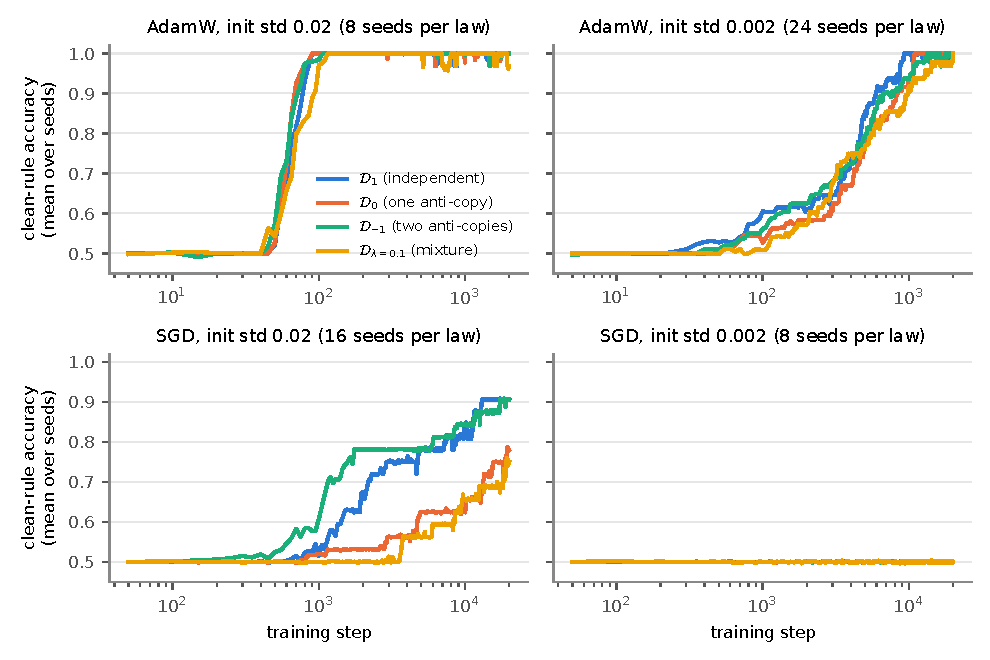
\includegraphics[width=0.9\linewidth]{figures/standard_transformer.pdf}
\caption{A standard two-layer Transformer separates the laws only under SGD. Mean clean-rule accuracy over seeds for the four laws,
AdamW and SGD at two initialization scales.}
\label{fig:standard}
\end{figure}

\section{Experimental results in detail}
\label{app:experiments}
\paragraph{Does the network produce the derived gradients?}
We first instantiate the matrices and residual paths of \cref{sec:architecture}, rather than directly coding its reduced logit.
Across 72 configurations spanning three context sizes, four cancellation coefficients, two losses, and three score/weight settings,
autograd agrees with the analytical logits and velocities to absolute tolerance $10^{-12}$.
This checks both the neural realization and the factor of two arising from the two trainable score groups.
All supported prefixes and errors are enumerated with their exact masses, so there is no sampling variability (\cref{app:network-experiments}).
The flow itself can also be run through the network: we integrate the four tied coordinates $(q_s,q_d,r_1,r_2)$ along
$-\nabla\mathcal L$ computed by automatic differentiation through the explicit matrices, by DOP853 (relative tolerance $10^{-10}$), from \cref{eq:initialization} until
source attention reaches $\tfrac12$. For $N=16$, $\kappa\in\{1,0\}$, $\varepsilon\in\{0.03,0.01,0.003\}$ and both losses, the $12$ routing times agree with the reduced
flow to relative error at most $1.9\times10^{-9}$, and $r_1-r_2$ and $q_s+q_d$ stay below $5\times10^{-14}$, so the reduced trajectories are those of the network.
The same check runs the causal model of \cref{thm:causal}: correlation loss averaged over the $N$ supervised prefixes, the flow stopped when every prefix routes.
For $N\in\{8,16\}$, the clean, independent and cancelling regimes ($\eta=0.2$ for the noisy ones) and $\varepsilon\in\{0.03,0.01\}$, the $12$ routing times agree with the reduced
causal flow to relative error at most $2\times10^{-11}$.

\paragraph{Matched loss comparison.}
\Cref{tab:network-flow} reports continuous gradient-flow times at error probability $0.1$.
The initialization, context size, population law, stopping rule and parameter metric are held fixed between the two losses.
The correlation runs test \cref{thm:separation}(i)--(ii); the cross-entropy runs test the escape orders of \cref{thm:separation}(iv)
and the complete routing that we verify only numerically.
\Cref{fig:network-flow} separately displays escape to score gap $0.01$ and routing to source attention $\tfrac{1}{2}$.

\begin{table}[t]
\centering\small
\caption{Matched population-flow experiment in the derived one-block parameterization.
Error probability $\eta=0.1$. Subscripts $1$ and $0$ denote the independent law $\Dlaw1$ and the anti-copy law $\Dlaw0$.
All columns are continuous gradient-flow time.}
\label{tab:network-flow}
\fitwidth{\begin{tabular}{@{}rr rrrr@{}}
\toprule
$N$ & $\varepsilon$ & $T_{\mathrm{corr},1}$ & $T_{\mathrm{corr},0}$ & $T_{\mathrm{ce},1}$ & $T_{\mathrm{ce},0}$\\
\midrule
16 & 0.03 & 133.1 & 1,380.0 & 140.9 & 1,406.8\\
16 & 0.01 & 176.9 & 4,316.4 & 184.8 & 4,351.2\\
16 & 0.003 & 225.0 & 14,655.1 & 232.9 & 14,698.7\\
16 & 0.001 & 269.0 & 44,248.7 & 276.9 & 44,300.3\\
64 & 0.03 & 520.6 & 5,480.0 & 546.4 & 5,593.7\\
64 & 0.01 & 695.9 & 17,214.8 & 721.7 & 17,363.5\\
64 & 0.003 & 888.5 & 58,557.6 & 914.3 & 58,745.0\\
64 & 0.001 & 1,064.3 & 176,921.0 & 1,090.1 & 177,143.8\\
\bottomrule
\end{tabular}
}
\end{table}
\begin{figure}[t]
\centering
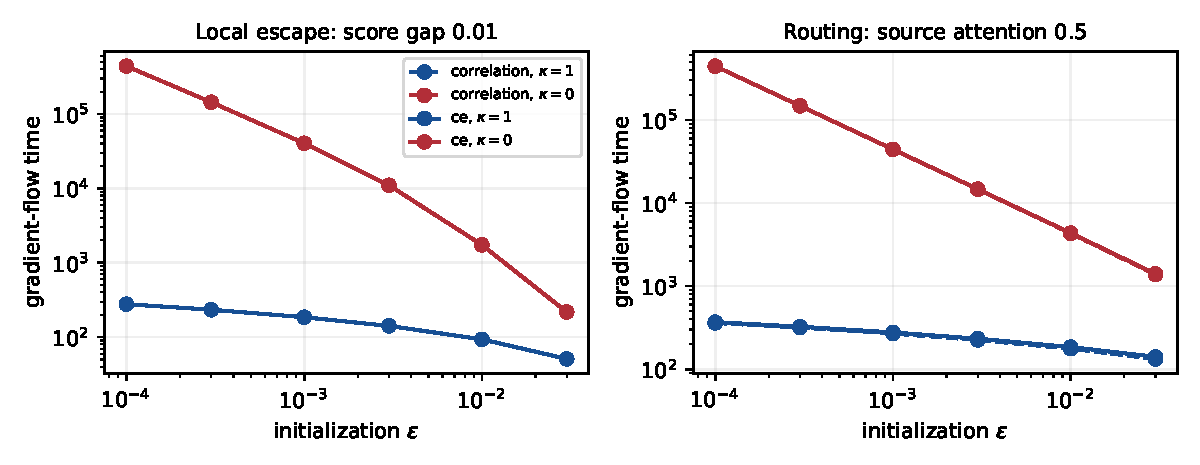
\includegraphics[width=\linewidth]{figures/one_block_scaling.pdf}
\caption{Separate tests of escape and full routing. Context size $N=16$, error probability $\eta=0.1$.
Dashed curves use correlation loss and solid curves use cross-entropy, with otherwise matched settings.
The theorem predicts distinct initialization orders for both local escape and complete routing.}
\label{fig:network-flow}
\end{figure}

\paragraph{The exact quadrature.} Direct integration of the flow of \cref{lem:invariant} agrees with \cref{eq:time} to five significant
figures, and the conserved quantity drifts by at most $6\times10^{-9}$, for $N\in\{16,64,256\}$ and $\varepsilon\in\{10^{-2},10^{-3}\}$;
every bound of \cref{thm:separation} holds (\cref{tab:quadrature}). Over-cancellation follows the exact criterion of
\cref{thm:separation}(iii): at $N=64$ and $\varepsilon=0.01$, routing completes at $\kappa=-0.007$, where $-F(q_0)<\varepsilon^2$, and does not
complete at $\kappa=-0.0283$, where $-F(q_0)\simeq3.9\times10^{-4}>\varepsilon^2$. The routing time is linear in $N$ under both laws. Reducing
$\varepsilon$ tenfold multiplies $\Tr(\Dlaw0)$ by $10.3$ and $\Tr(\Dlaw1)$ by $1.5$.

\begin{figure}[t]
\centering
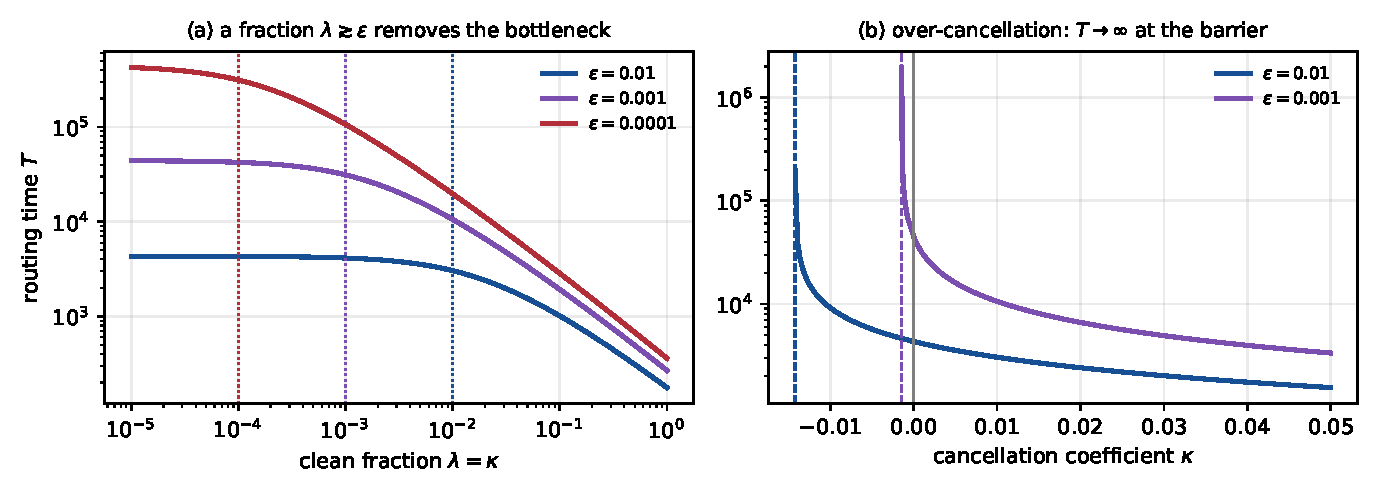
\includegraphics[width=\linewidth]{figures/kappa_sweep.pdf}
\caption{Routing time across the cancellation coefficient, correlation loss, $N=16$, $\eta=0.1$, exact quadrature.
(a) Diluting the anti-copy law with a clean fraction $\lambda=\kappa$: the plateau at $\Theta(\tfrac{1}{\varepsilon})$ ends near $\lambda\approx\varepsilon$ (dotted lines).
(b) Through $\kappa=0$ into over-cancellation: the routing time diverges at the barrier $\varepsilon^2=-F(q_0)$ (dashed lines), at $\kappa\approx-1.4\,\varepsilon$.}
\label{fig:kappa}
\end{figure}

\paragraph{Diluting the cancellation.} We integrate the primitive and the routing time together for $\kappa\in[-1,1]$ (\cref{fig:kappa}).
For clean fractions $\lambda\in[0,1]$, $N\in\{16,64\}$ and $\varepsilon\in\{10^{-2},10^{-3},10^{-4}\}$, the exact routing time stays within a factor $1.03$--$1.51$ of
$\tfrac{N-1}{\gamma}\int_0^1\tfrac{dq}{\varepsilon^2+\lambda q+q^2}$, the quantity that \cref{cor:dilution} evaluates. At $N=16$ the over-cancellation barrier sits at
$\kappa=-0.0142$ for $\varepsilon=10^{-2}$ and at $\kappa=-0.00141$ for $\varepsilon=10^{-3}$.

\begin{table}[t]
\caption{Exact routing times of the correlation-loss flow. $\gamma=1$. ODE: direct integration; quadrature: \cref{eq:time}; drift:
largest deviation of $r^2-F(q)-\varepsilon^2$ along the trajectory.}
\label{tab:quadrature}
\centering\small
\begin{tabular}{@{}rr rr rr r@{}}
\toprule
 & & \multicolumn{2}{c}{$\Dlaw1$} & \multicolumn{2}{c}{$\Dlaw0$} & \\
\cmidrule(lr){3-4}\cmidrule(lr){5-6}
$N$ & $\varepsilon$ & ODE & quadrature & ODE & quadrature & ratio\\
\midrule
16  & $10^{-2}$ & 141.5  & 141.5  & 3{,}453   & 3{,}453   & 24\\
16  & $10^{-3}$ & 215.2  & 215.2  & 35{,}399  & 35{,}399  & 164\\
64  & $10^{-2}$ & 556.8  & 556.8  & 13{,}772  & 13{,}772  & 25\\
64  & $10^{-3}$ & 851.4  & 851.4  & 141{,}540 & 141{,}540 & 166\\
256 & $10^{-2}$ & 2{,}215 & 2{,}215 & 55{,}043  & 55{,}043  & 25\\
256 & $10^{-3}$ & 3{,}394 & 3{,}394 & 566{,}080 & 566{,}080 & 167\\
\bottomrule
\end{tabular}
\end{table}

\paragraph{Does the causal error process match the new theorem?}
The causal check propagates the exact finite-state law of the prefix sum and final sign.
For $\eta=0.2$ and $N\in\{8,16,32\}$, it checks every supervised position's local error rate, cancellation coefficient, and the cancelling variance recurrence.
Propagating the error count jointly with these states also verifies the binomial law and the high-probability bound.
An additional 18 matrix-gradient configurations enumerate both instructions and both error signs under the history-dependent kernel.
The largest gradient discrepancy is below $10^{-12}$; there is no Monte Carlo estimation.
\Cref{tab:causal-flow} reports 36 averaged-loss routing runs across fully correct, independently corrupted and structured corrupted supervision.
All three share the initialization, seed and instruction process; the two noisy regimes share $\eta=0.2$.
Nine further matrix configurations verify the fully correct control.
The independent-noise times agree with $T_{\mathrm{clean}}/(1-2\eta)$ to relative error below $10^{-10}$.
The expected incorrect fraction is $0.1125$, $0.10625$, and $0.103125$ for $N=8,16,32$, respectively, approaching $0.1$.
For $N=16$, reducing $\varepsilon$ from $0.01$ to $0.001$ increases routing time by a factor $1.52$ with independent errors and $10.26$ with cancelling errors.
All runs satisfy the explicit bounds in \cref{app:trace-proof}.
At $N=16$ and $\varepsilon=0.01$, eight additional runs sweep $\eta\in\{0.1,0.2,0.3,0.4\}$ in the two noisy regimes.
The rescaled times $(1-2\eta)T$ remain constant to relative error below $10^{-10}$: about $207.9$ for independent errors and $5{,}089.6$ for structured errors.

\begin{table}[t]
\centering\small
\caption{Correct computation from clean and corrupted reasoning supervision. The clean control has no errors; both noisy regimes have local error rate $\eta=0.2$.
The same block parameters train on all $N$ selected positions. Times reach source attention $\tfrac{1}{2}$ on every prefix; the final column compares structured errors with clean supervision.}
\label{tab:causal-flow}
\begin{tabular}{@{}rr rrrr@{}}
\toprule
$N$ & $\varepsilon$ & clean & independent & structured & ratio to clean\\
\midrule
8 & 0.03 & 81.3 & 135.6 & 1,393.2 & 17.1\\
8 & 0.01 & 107.8 & 179.7 & 4,347.9 & 40.3\\
8 & 0.003 & 136.8 & 228.1 & 14,747.2 & 107.8\\
8 & 0.001 & 163.4 & 272.3 & 44,511.6 & 272.5\\
16 & 0.03 & 156.1 & 260.2 & 2,708.0 & 17.3\\
16 & 0.01 & 207.9 & 346.5 & 8,482.6 & 40.8\\
16 & 0.003 & 264.7 & 441.2 & 28,819.0 & 108.9\\
16 & 0.001 & 316.6 & 527.6 & 87,034.8 & 274.9\\
32 & 0.03 & 305.2 & 508.7 & 5,336.7 & 17.5\\
32 & 0.01 & 407.5 & 679.2 & 16,752.4 & 41.1\\
32 & 0.003 & 519.9 & 866.5 & 56,967.0 & 109.6\\
32 & 0.001 & 622.5 & 1,037.5 & 172,097.6 & 276.5\\
\bottomrule
\end{tabular}

\end{table}

\paragraph{Does the separation survive untying?}
We next train every entry of the one-block network independently: all seven-by-seven query, key, value and output matrices,
both MLP layers with their bias, and the readout, under binary cross-entropy on the exact population of $\Dlaw\kappa$, $N=16$, $\eta=0.1$.
Three initialization families move progressively away from the theorem.
(A) The directions of \cref{sec:architecture} with random magnitudes: fixed directions get magnitudes in $[\tfrac{1}{2},2]$,
each of the eight MLP rule entries gets $\varepsilon$ times a magnitude in $[\tfrac{1}{2},2]$, with a random sign per layer, and the four MLP units are no longer tied.
(B) The same plus independent Gaussian noise of fan-in scale $0.1$ or $0.3$ on every matrix.
(C) Fan-in Gaussian matrices scaled by $\varepsilon$, a sixteen-unit MLP, and nothing hand-coded.
Full-batch gradient descent with backtracking measures time on the gradient-flow clock (\cref{app:network-experiments}).

\Cref{tab:untied} reports how many of three seeds reach $99\%$ clean-rule accuracy within flow time $3\times10^4$.
With clean supervision, every seed of family (B) learns at every $\varepsilon\le0.1$, within $51$ time units,
and two of three seeds of family (A) learn at every $\varepsilon\le0.5$; the third starts with opposite rule-factor signs in the two MLP layers and fails at every $\varepsilon$.
Exact cancellation stalls: with noise, no seed learns below $\varepsilon=0.1$ ($0.1$ noise) or $\varepsilon=0.5$ ($0.3$ noise);
without noise, the seeds that learn slow down roughly as $\tfrac{1}{\varepsilon}$, from $24$ time units at $\varepsilon=0.3$ to $2{,}514$ at $\varepsilon=0.003$.
Over-cancellation fails at every $\varepsilon\le0.3$ and recovers only at $\varepsilon\ge0.5$ ($\varepsilon=1$ with $0.3$ noise),
the untied counterpart of the barrier in \cref{thm:separation}(iii).
In family (C), with three seeds and gradient descent, the three laws do not separate clearly; the next paragraph tests this regime at scale.

\paragraph{Does the full-matrix plateau appear?}
We train every entry from exactly $W_0$, $N=16$, $\eta=0.1$, by gradient descent with step $0.5$, and records the first flow time at which
$\|W-W_0\|_F=\varepsilon$. Under the anti-copy law the exit time is $1{,}048$, $1{,}579$, $3{,}170$, $6{,}351$, $10{,}592$ and $15{,}893$ for
$\varepsilon=0.03,0.02,0.01,0.005,0.003,0.002$, that is between $31.4/\varepsilon$ and $31.8/\varepsilon$, and the largest $|\E[yz_W]|$ inside the ball is $0.065\,\varepsilon^3$ at every $\varepsilon$:
the order of \cref{thm:fullmatrix}, with a much smaller constant than the proved $\gamma C_B=528$. Under the independent law every run leaves the ball at flow time $23$,
whatever $\varepsilon$ is, and its correlation inside the ball scales as $\varepsilon^2$. The full-matrix network can therefore escape quickly when credit is not cancelled.
A variant pads the embeddings and $W_0$ with zeros to residual width $D$ and trains every $D$-dimensional matrix.
From exactly $W_0$ the padded coordinates receive zero gradient and stay zero, so widths $16$ and $64$ reproduce the numbers above exactly.
A second variant starts instead from $W_0$ plus a Gaussian perturbation of Frobenius norm $\varepsilon^{3/2}$ spread over every entry, padded ones included,
the setting of \cref{thm:fullmatrix}(iii). At widths $7$, $16$ and $64$, the anti-copy law then leaves the ball at flow time between $20.2/\varepsilon$ and $26.5/\varepsilon$,
the largest $|\E[yz_W]|$ inside it is at most $0.105\,\varepsilon^3$, and the independent law still leaves at flow time $22.5$--$23$ for every $\varepsilon$.

\paragraph{From fully random initialization.}
We repeat family (C) with ten seeds, $N\in\{8,16,32\}$, $\varepsilon\in\{0.05,0.1,0.2,0.3,0.5,0.7,1,1.5\}$, and two optimizers: backtracking gradient descent with
flow-time budget $10^5$, and Adam with step size $3\times10^{-3}$ for $10^5$ steps (\cref{tab:randinit}).
The first escape from chance takes the same time under every law (for Adam, a median of $45$, $52$ and $60$ steps at $N=8,16,32$, within a few steps across $\kappa$):
from random matrices it is limited by the product of small weights, not by the data, as in deep linear networks.
The laws differ in where training goes next. With Adam, all $240$ runs on the independent law reach the Bayes predictor; on the anti-copy law $33$--$40\%$ of runs
stall, and with two anti-copies $43$--$50\%$. All $195$ stalled runs are flat, with loss changing by less than $10^{-4}$ over the last $4\times10^4$ steps, and $193$ of them sit at a single stationary point
for each law and context size, with loss $0.43$--$0.50$ against the Bayes value $0.325$ and clean accuracy $79$--$91\%$. Gradient descent shows the same ordering among initializations $\varepsilon\ge0.5$, where the
independent law learns reliably. From random initialization, then, cancellation does not delay the first escape; it makes training land in a worse stationary point.
At every stalled point the mean source attention is $\tfrac12$. The point routes by instruction: when one sign of $b$ is shown, attention is on the source and the
loss is $H(\eta)$, with $H$ the binary entropy in nats; when the other is shown, the source receives no weight and the readout is the Bayes predictor of $y$ from the decoys alone. The clean accuracy is then
$\tfrac12(1+a_{\mathrm{dec}})$ and the loss $\tfrac12(H(\eta)+H(y\mid\text{decoys}))$, where $a_{\mathrm{dec}}$ is the best decoy-only accuracy. For one anti-copy these give $82.8$, $80.2$ and
$78.6\%$ with losses $0.485$, $0.498$ and $0.504$ at $N=8,16,32$; for two anti-copies, $90.6$, $85.5$ and $82.2\%$ with $0.426$, $0.468$ and $0.489$. Every
value equals the measured one to three decimals. Under the independent law the decoys carry no information about the source, so this split point gives no decoy-side
gain, consistent with no independent-law run stalling.

\paragraph{Removing the product of small weights.} Family (C$'$) keeps every matrix random but draws the query, value and output matrices at order one,
$\mathrm N(0,\tfrac{1}{\text{fan-in}})$, and only the key and both MLP layers at $\varepsilon Z/\sqrt{\text{fan-in}}$, so attention starts uniform up to $O(\varepsilon)$;
the MLP bias is either the gate value $-B$ or uniform on $\pm\tfrac{1}{\sqrt7}$, and the readout has scale $1$ or $\varepsilon$
(same $N$, $\varepsilon$, seeds and optimizers as \cref{tab:randinit}). The plateau exit again takes the same time under
every law, and it does not grow as $\varepsilon$ shrinks (at $N=16$ with gradient descent, flow time $28$--$36$ at $\varepsilon=0.05$ for all three laws), so this rescaling does not
recover the $\tfrac{1}{\varepsilon}$ delay of \cref{thm:separation}. With the random bias the laws again differ in how often training reaches $99\%$ clean-rule accuracy:
with Adam, $79$--$80$ of $80$ runs per cell under the independent law, $27$--$43$ under one anti-copy and $19$--$28$ under two. With the gate bias all three laws learn
in only $21$--$39$ of $80$.

\begin{table}[t]
\centering\small
\caption{Fully random initialization, every matrix entry trained. Anti-copy law, $\eta=0.1$, binary cross-entropy, ten seeds per initialization.
Each cell: runs reaching $99\%$ clean-rule accuracy within the budget; Adam pools eight initializations, gradient descent the four with $\varepsilon\ge0.5$.}
\label{tab:randinit}
\begin{tabular}{@{}lcccccc@{}}
\toprule
 & \multicolumn{3}{c}{Adam, all $\varepsilon$} & \multicolumn{3}{c}{GD, $\varepsilon\ge0.5$}\\
\cmidrule(lr){2-4}\cmidrule(lr){5-7}
$N$ & $\kappa=1$ & $\kappa=0$ & $\kappa=-1$ & $\kappa=1$ & $\kappa=0$ & $\kappa=-1$\\
\midrule
8 & 80/80 & 54/80 & 45/80 & 37/40 & 24/40 & 20/40\\
16 & 80/80 & 52/80 & 46/80 & 34/40 & 23/40 & 19/40\\
32 & 80/80 & 48/80 & 40/80 & 33/40 & 23/40 & 19/40\\
\bottomrule
\end{tabular}

\end{table}

\begin{table}[t]
\centering\small
\caption{Untied one-block training under the anti-copy law. Every matrix entry trains; binary cross-entropy, $N=16$, $\eta=0.1$.
Each cell: seeds (of three) reaching $99\%$ clean-rule accuracy within gradient-flow time $3\times10^4$, and their median time.
$\kappa=1$: independent decoys; $\kappa=0$: one anti-copy; $\kappa=-1$: two anti-copies.}
\label{tab:untied}
\fitwidth{\begin{tabular}{@{}llcccccc@{}}
\toprule
Initialization & $\kappa$ & $\varepsilon=0.003$ & $\varepsilon=0.03$ & $\varepsilon=0.1$ & $\varepsilon=0.3$ & $\varepsilon=0.5$ & $\varepsilon=1$\\
\midrule
A: directions & $+1$ & 2/3 (85) & 2/3 (59) & 2/3 (34) & 2/3 (14) & 2/3 (9) & 1/3 (4)\\
 & $+0$ & 1/3 (2,514) & 2/3 (497) & 2/3 (114) & 2/3 (24) & 1/3 (9) & 1/3 (4)\\
 & $-1$ & 0/3 & 0/3 & 0/3 & 0/3 & 1/3 (26) & 1/3 (4)\\
\addlinespace
B: $+\,0.1$ noise & $+1$ & 3/3 (51) & 3/3 (44) & 3/3 (34) & 2/3 (14) & 2/3 (8) & 2/3 (57)\\
 & $+0$ & 0/3 & 0/3 & 1/3 (97) & 1/3 (20) & 1/3 (10) & 1/3 (4)\\
 & $-1$ & 0/3 & 0/3 & 0/3 & 0/3 & 2/3 (454) & 1/3 (5)\\
\addlinespace
B: $+\,0.3$ noise & $+1$ & 3/3 (34) & 3/3 (34) & 3/3 (30) & 3/3 (20) & 3/3 (11) & 2/3 (19)\\
 & $+0$ & 0/3 & 0/3 & 0/3 & 0/3 & 1/3 (20) & 1/3 (6)\\
 & $-1$ & 0/3 & 0/3 & 0/3 & 0/3 & 0/3 & 1/3 (11)\\
\addlinespace
C: random & $+1$ & 0/3 & 0/3 & 1/3 (26,330) & 1/3 (1,009) & 2/3 (168) & 3/3 (44)\\
 & $+0$ & 0/3 & 0/3 & 1/3 (23,109) & 1/3 (885) & 1/3 (211) & 2/3 (21)\\
 & $-1$ & 0/3 & 0/3 & 1/3 (23,109) & 1/3 (885) & 1/3 (185) & 2/3 (22)\\
\bottomrule
\end{tabular}
}
\end{table}
